\documentclass{article}
\usepackage[utf8]{inputenc}
\usepackage[]{graphicx}
\usepackage[letterpaper, margin=1in]{geometry}
\usepackage{hyperref}
\usepackage{pdflscape}
\usepackage{pdfpages}
\usepackage{setspace}
\usepackage{amsmath}
\doublespacing



\usepackage[style=verbose-note,doi=false,isbn=false,url=false,firstinits=true,backend=biber]{biblatex}
\renewbibmacro{in:}{%
  \ifentrytype{article}{}{\printtext{\bibstring{in}\intitlepunct}}}

\renewcommand*{\multicitedelim}{\iffootnote{\newline}{\addsemicolon\space}}
\renewcommand{\bibfootnotewrapper}[1]{\bibsentence #1}
\usepackage{scrextend}
\deffootnote{1.7em}{1em}{\textsuperscript{\thefootnotemark}}

\addbibresource{bibliography.bib}

\usepackage{chngcntr}
\counterwithin{figure}{section}

\newcommand{\beginsupplement}{%
% \setcounter{table}{0}  \renewcommand{\thetable}{A\arabic{table}}     \setcounter{figure}{0} \renewcommand{\thefigure}{A\arabic{figure}}
\setcounter{section}{0} \renewcommand{\thesection}{A\arabic{section}}
}


\title{Forecasting Technology Performance: Initial Tests with Time Series Extrapolation and Patent Data}
\author{Jeff Alstott}
\date{August 2017}

\begin{document}

\maketitle

\textit{This research is based upon work supported in part by the Office of the Director of National Intelligence (ODNI), Intelligence Advanced Research Projects Activity (IARPA). The views and conclusions contained herein are those of the authors and should not be interpreted as necessarily representing the official policies, either expressed or implied, of ODNI, IARPA, or the U.S. Government. The U.S. Government is authorized to reproduce and distribute reprints for governmental purposes notwithstanding any copyright annotation therein.}

\pagebreak

\tableofcontents

\section{Overview}
This report describes principles of trend extrapolation for a lay audience (without equations) and shows how different kinds of trend extrapolation worked on historical data of technology trends. We ask the question ``Which methods would have allowed me to better predict the future, if I had been standing in 1990?" With the presently available data, the simplest models performed best.

This study had 3 tasks:
\begin{enumerate}
    \item Create statistical software to enable principled extrapolation of technology trends, including forecasts with correctly-stated uncertainty\label{software_goal}.
    \item Test what kinds of trend extrapolation would have best predicted past technology performance data\label{extrapolation_goal}.
    \item Test if using patent data could have improved predictions of technology performance data\label{patent_goal}.
\end{enumerate}

The software for task \ref{software_goal} has been written, rigorously tested and made publicly available.\footnote{\url{https://github.com/jeffalstott/pystan_time_series}} The software was used to perform task \ref{extrapolation_goal} and \ref{patent_goal}, the results of which are described here. Task \ref{patent_goal} was unlikely to work, given noisy historical data, and in fact it didn't. However, the analysis pipeline that was created is now ready for any cleaner data that may be assembled in the future. This study thus provides the tools and examples for future forecasters to make better predictions of technology.

More technical details about the models, software and data are included at the end of this report. They are presented in a form designed to be useful for those looking to implement these methods, and all code used in this study is available online\footnote{\url{https://github.com/jeffalstott/technologytimeseries_forecasting}}.

\section{Forecasting Technology Trends}
Consider a technology, such as electronic computers. We care about computers because they provide capabilities (e.g. processing information) given some resources (e.g. time, energy or dollars).  Forecasting technologies' capability per unit resource is the object of interest for this study. For example, say we will have \$1,000 to buy a computer in 2030; how many instructions per second will that computer be able to calculate? A simple way make a forecast is trend extrapolation: look at historical data, identify a trend, and draw the trend out to the future date. In the case of electronic computers, we can observe historical data from the 1940s until today (Fig. \ref{fig:trend_extrapolation_example}A). What trend do we identify?

\begin{figure}
    \centering
    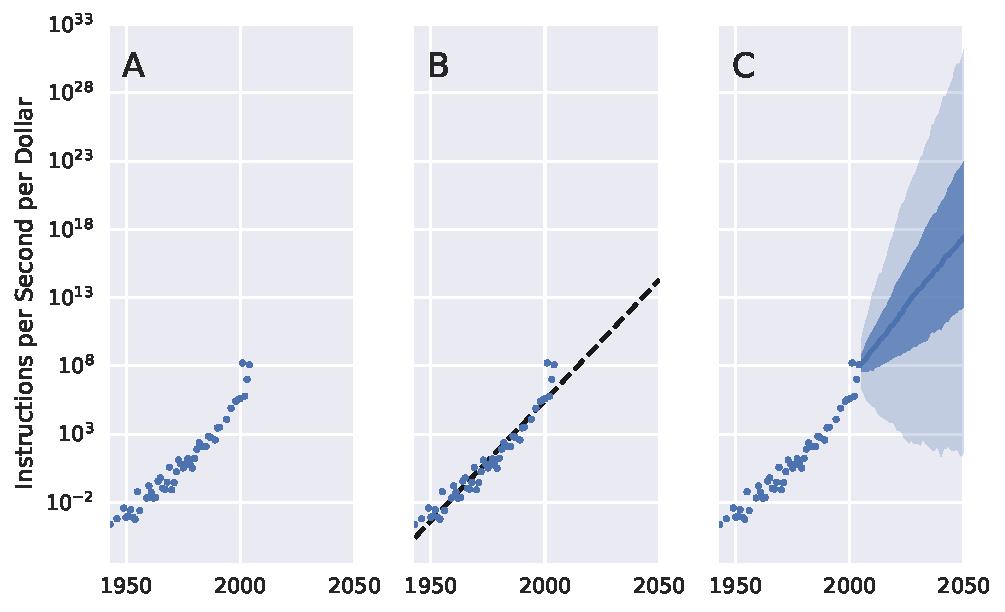
\includegraphics[width=.75\textwidth]{figs/trend_extrapolation_example.pdf}
    \caption{\textbf{Extrapolating technology trends with different methods.} A) Historical prices of computing power B) Using linear regression to forecast future computing power C) Using Bayesian trend extrapolation methods to make probabilistic forecasts. Light band: 95\% confidence interval. Dark band: 50\% confidence interval. Line: Median forecast.}
    \label{fig:trend_extrapolation_example}
\end{figure}

\subsection{Making uncertain forecasts}\label{forecasting_basics}
The simplest and most common trend extrapolation technique is to literally draw a line through the data points, perhaps through linear regression, and find an answer: $5.8*10^{13}$ (Fig. \ref{fig:trend_extrapolation_example}B). This process is fast, but unfortunately it has several downsides, chief among them that it's wrong. That \textit{exact} predicted performance will virtually certainly not happen. A better forecast would give statements with uncertainties, like this: 
\begin{itemize}
    \item $1.9*10^5 - 4.7*10^{25}$: 95\% probability
    \item $3.7*10^{12} - 6.0*10^{19}$: 50\% probability
\end{itemize}

A forecast like the one in Fig. \ref{fig:trend_extrapolation_example}C not only gives predictions, but uncertainties about those predictions (the broader, lighter band is the 95\% confidence interval, and the narrower, darker band is the 50\% confidence interval). This is a forecast that can be well-calibrated, if done well - observed events should be in the 95\% confidence interval 95\% of the time. This is a forecast that is operationally useful, as opposed to a point prediction that is virtually guaranteed to be correct 0\% of the time. 

Methods to do trend extrapolation with probabilistic forecasts are well-studied and well-used, particularly in finance. As such, people have developed countless possible descriptions for a trend (such trends are often called ``models"). For example, perhaps the simplest model is this: ``every year the technology improves by a fixed amount, but each year there is some random noise around that improvement." One possible interpretation of such a model is that the fixed improvement rate is due to something innate about the technology itself, while the noise each year is due to other factors like economic conditions, random chance that a certain pair of inventors meet each other in the hallway, etc. A somewhat more complex model could be: ``every year the technology improves by a fixed amount, and each year there is some noise around that improvement, but the effects of last year's noise are also still felt a small amount." Such a model would just be adding the concept that the shock of, say, an economic recession could last for more than one year. In both cases, the uncertainty about what the future holds is because of the noise; we might know what the general shape of the noise is like on average, but we don't know what the precise effect of the noise will be each year. The effects of this noise accumulates, which is why our predictions' confidence intervals get wider as we forecast further into the future (Fig. \ref{fig:trend_extrapolation_example}C).

\subsection{Uncertainty in our knowledge: Bayesian statistics}
While trend extrapolation techniques have been around for many years, only recently have researchers started to apply these methods to historical technology trends.\footcite{Farmer2016} The most recent research is a good start (and heavily inspired the present study), but there are opportunities for further advancement. One way to better understand historical trends, and thus make even better forecasts, is to understand our uncertainty even better. In the above paragraph, we considered a model in which there's a fixed improvement every year, but it's the random noise that is causing our forecasts to be imprecise. This might be a true story about the world, but it's an incomplete story about our knowledge of that world. A more complete story is that we think the technology improves a fixed amount each year, \textit{but we don't even know for certain what that fixed amount is}. Thus, our forecasts should not only take into account our uncertainty on the future random noise, but should also take into account our uncertainty about the size of the fixed improvement every year\footnote{We can even take into account our uncertainty in the average shape of the noise}. Our forecasts can now combine two sources of uncertainty: the uncertainty of what values random variables will produce each year \textit{and} our uncertainty of what value fixed variables have across all years. The forecasts in Figure \ref{fig:trend_extrapolation_example}C do this, as will all forecasts in this study. The method for describing our uncertainty of the parts of the model is called Bayesian statistics, and the principle is simple: 
\begin{enumerate}
    \item Start with some prior belief on what the values of the parts of the model could be. In lieu of any prior knowledge, these should be broad, diffuse beliefs, like ``Somewhere between zero and a million, but somewhat higher probability around a thousand."\label{bayes_P(M)}
    \item Look at historical data, and consider how likely that data would have been had the parts of the model had different values\label{bayes_P(D|M)}.
    \item Combine parts \ref{bayes_P(M)} and \ref{bayes_P(D|M)} to update to the data-driven, ``posterior" belief of what the values of the parts of the model are.
\end{enumerate}

This process is shown for some simulated data in Figure \ref{fig:bayesian_updating}. As we add more data our posterior belief gets tighter and tighter around the true value, but we never have complete certainty in the values of the parts of the model.\footnote{A nice property of this method is that if we don't have much data, we're not entirely stuck: we can rely on our prior belief to make predictions. We will see the merits of this later in sections \ref{partial_pooling_section} and \ref{Atari_section}}

\begin{figure}
    \centering
    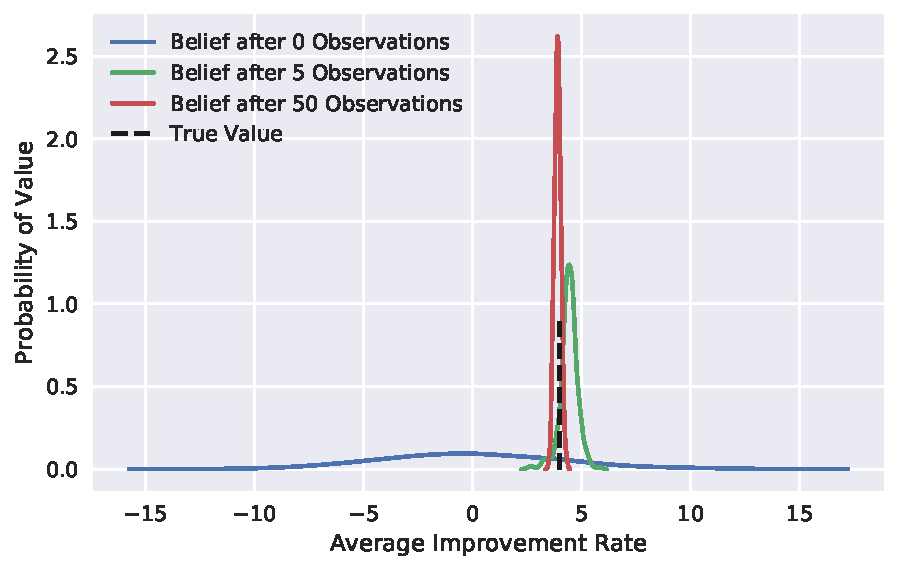
\includegraphics[width=.75\textwidth]{figs/bayesian_updating.pdf}
    \caption{\textbf{Bayesian inference of an unknown parameter.} A technology trend was simulated with an average yearly improvement rate, but with noise that could raise or lower the improvement each individual year. Before observing any data, we started with a broad prior belief as to what the average improvement rate could be. After observing just 5 years of data, the belief tightened towards the true value, and after 50 years of observation the belief was tightly centered on the true value.}
    \label{fig:bayesian_updating}
\end{figure}

\subsection{Uncertainty in our models: model comparison}
We also have uncertainty not just about the values of parts of a model, but on whether we're using the right model at all. Previously we considered two models: both had noise every year, but in one model the noise had some influence on the next year as well. We are uncertain about which model better describes the data.\footnote{Sometimes we're very confident about what model or description of the data is right, because we know what the underlying mechanisms are in the system we're studying, but even that confidence is effectively built out of observing lots of historical data.} It's possible to combine both models into a single model, and then make forecasts that incorporate our uncertainty as to which model is correct.\footnote{In this specific case, the second model does this automatically: the only difference is in the influence of noise a year later, so if the data suggests that influence is 0, that indicates the first model better describes the data.} 

If we want to get more certainty as to which model is correct, we can test them, by seeing which  better predicts future data. This is the central activity of this study: we compared the forecasting power of several kinds of models. Each model's values were determined, with Bayesian statistics, by using historical data up to a given year (specifically, 1990), and then that model was used to forecast ``future" data (from 1991 to 2013). Those models that better predicted the future data are more likely to be useful in predicting further future data, including data from new technologies.

It is worth noting that comparing models is no guarantee that any of the models will be any good. Some of the technology trends examined here are forecasted very well by the models tested, but others are far off. This may sometimes be because there was just insufficient data to infer the right values for the model. More often, it's because the model is very wrong. Seeing such discrepancies and proposing new models to try is the job for the scientist. This is what led us to try to expand on simple trend extrapolation models with patent data.\footnote{It didn't work.}

\subsection{Evaluating forecasts}
Comparing model's forecasts requires scoring how good each forecast was. In an ideal operational context, we would have some operational consequence for more or less accurate forecasts (e.g. dollars saved). This would let us say ``A forecast that is off by this much is worth \$$X$, and a forecast that is off by that much is worth \$$Y$." Then for each forecasted data point, we can evaluate the value of the model's prediction and sum the values to cache out the model's accuracy in dollars. 

Without an operational context, we will score models' predictions of each forecasted data point using a more generic measure. First, for each forecasted data point we calculate the model's predicted probability density.\footnote{For continuous data, the probability for any specific predicted value is 0, but the probability \textit{density} around that value may be a positive number.} Then we take the log of that probability density. This log(probability density) is a standard in industry and academia for evaluating predictions of all kinds because it has justifications in information theory, but for present purposes it is sufficient to know that larger numbers are more accurate predictions. 

\begin{figure}
    \centering
    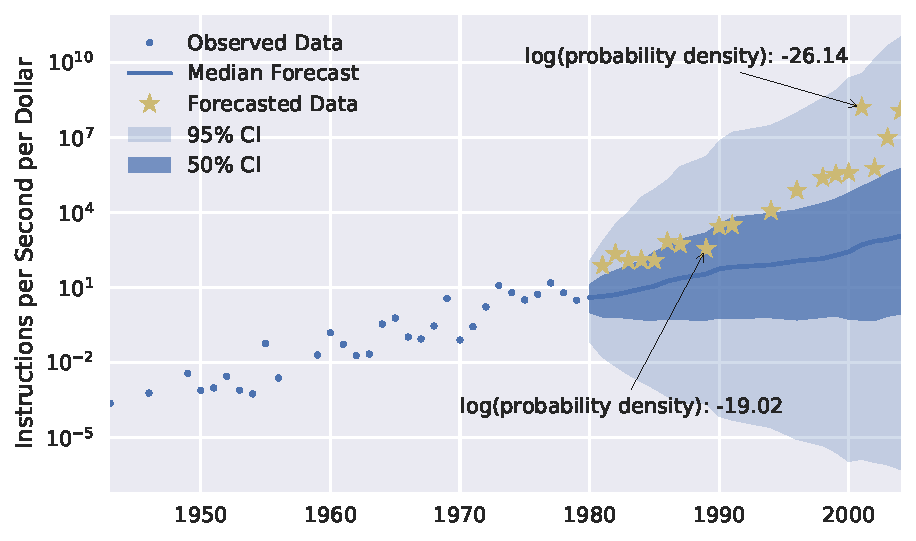
\includegraphics[width=.75\textwidth]{figs/forecast_evaluation.pdf}
    \caption{\textbf{Making and testing forecasts of technology.} Changes in the price of computer power were modeled using historical data up until 1980 (blue dots). This model made probabilistic forecasts of future prices (line and shaded region), which were then tested using subsequent historical data from 1981 onward (yellow stars). A forecast's accuracy for a given year was quantified as the log of the probability density of the true data for that year.}
    \label{fig:forecast_evaluation}
\end{figure}

Figure \ref{fig:forecast_evaluation} shows a set of forecasts and the log(probability densities) of those forecasts. We will summarize how well a model forecasts future data by simply averaging the log(probability density) of all forecasts it makes, across all technologies. Again, in an operational context this would not be appropriate; not all technologies are equally operationally important, so getting the predictions of some technologies better is more important than others. However, in the absence of an operational context to weight the different technologies, we will simply average them.

\section{Historical Data}
\begin{figure}
    \centering
    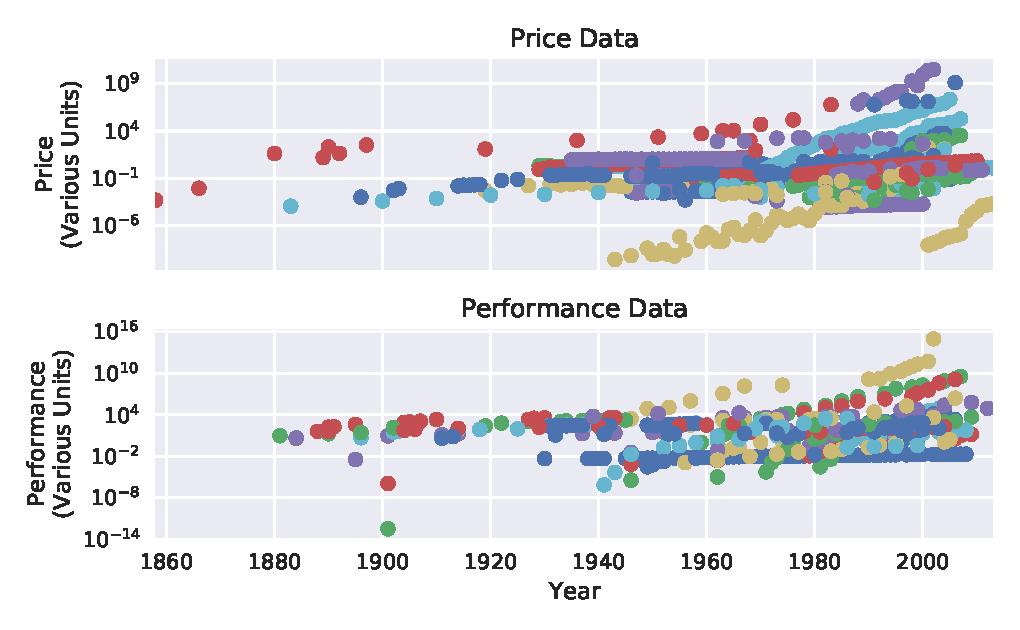
\includegraphics[width=.75\textwidth]{figs/Historical_Technology_Data.pdf}
    \caption{\textbf{The historical technology data used for creating and testing forecasts.} Top) Price data, in the form of the amount of capability per dollar. Bottom) Performance data, in the form of the amount of capability per some physical resource (e.g. computers' computations per joule, batteries' energy per kilogram, etc.)}
    \label{fig:Historical_Technology_Data}
\end{figure}

The historical technology data used in this study came from previously published articles \footcite{Farmer2016,Magee2016a,Nagy2013} and is hosted online at \url{https://github.com/jeffalstott/technologytimeseries}. These data included 130 different trends with a total of 2,204 data points (Fig. \ref{fig:Historical_Technology_Data}). Descriptions of all of these data are included in the Appendix (section \ref{time_series_metadata}). Each individual trend was for some technology (e.g. ``Batteries" or ``Ethylene") and the data was about some dimension of the quality of that technology (e.g. ``energy storage per kilogram" or ``kilograms per dollar"). A single technology could have multiple trends, with each trend reflecting a different dimension of quality. We separate these trends into two varieties:
\begin{enumerate}
    \item \textbf{Price}: the amount of currency to either purchase or produce a unit or output of the artifact at that moment in history (e.g. ``kilograms per dollar" or ``computations per dollar"). This number could go lower or higher over time. 
    \item \textbf{Performance}: the amount of functional output that the artifact could produce for some unit of input (e.g. ``energy storage per kilogram"). This data only reflects record-breakers, so the number is only able to go higher over time.
\end{enumerate}

Sometimes inventors patent their inventions, which leaves a public record of those inventions that may contain useful information for making forecasts. In this study, most (72) of the technology price and performance trends were accompanied by patent data. For these technologies, previous studies had identified/defined their functional ``domains," such as ``magnetic information storage" or ``genomics."\footcite{Benson2012,Benson2014} Patents were then found that related to these domains. These patents were identified using a system that begins with domain expert analysis of patent texts but then ends with domains defined through patent metadata. This metadata is curated by the US Patent \& Trademark Office for millions of patents, and so allowed the researchers to automatically match large numbers of patents with domains. These domains of patents can then be matched up with technology price and performance trends. Previous research has found that some patent features correlate with technologies' average improvement speed.\footcite{Benson2015,Triulzi2017} In the present study, we tested if this data could be used to improve forecasting. 

10 of the trends were questionable in some way, generally because it seemed the recorded data didn't actually reflect the stated measure (e.g. wrong order of magnitude) or the measure seemed ill-defined (e.g. one could increase the performance just by having two copies of the artifact next to each other). These trends were removed, leaving 120 trends with 2,022 data points (price: 1,565; performance: 457). These data are the shown in Figure \ref{fig:Historical_Technology_Data}.

\begin{figure}
    \centering
    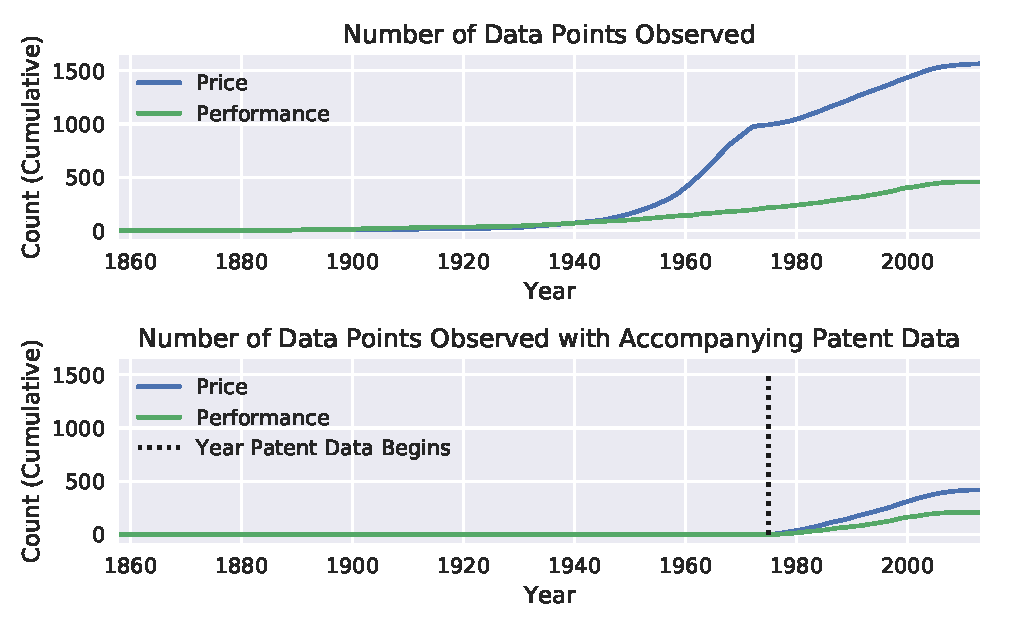
\includegraphics[width=.75\textwidth]{figs/Historical_Technology_Data_Cumulative.pdf}
    \caption{\textbf{The cumulative amount of historical data that had been observed by any possible training year.} Not all technology trends were paired with patent data, and digital patent records were only available staring in 1975.}
    \label{fig:Historical_Technology_Data_Cumulative}
\end{figure}

Forecasts were made through hindcasting - only data that appeared before a specific date was used to train the model, and then subsequent data that appeared after that date was forecasted. Thus a relevant question for training the model is not how much data there is in total, but how much existed before a given date. That is the amount of data that could be used to train a model on that date. The cumulative counts of the data are shown in Figure \ref{fig:Historical_Technology_Data_Cumulative}. Unfortunately, digitized patent data was only available after 1975. As such, technology trend data that had associated patent data only began at that date, and accumulated to a much smaller amount of total data. 

\begin{figure}
    \centering
    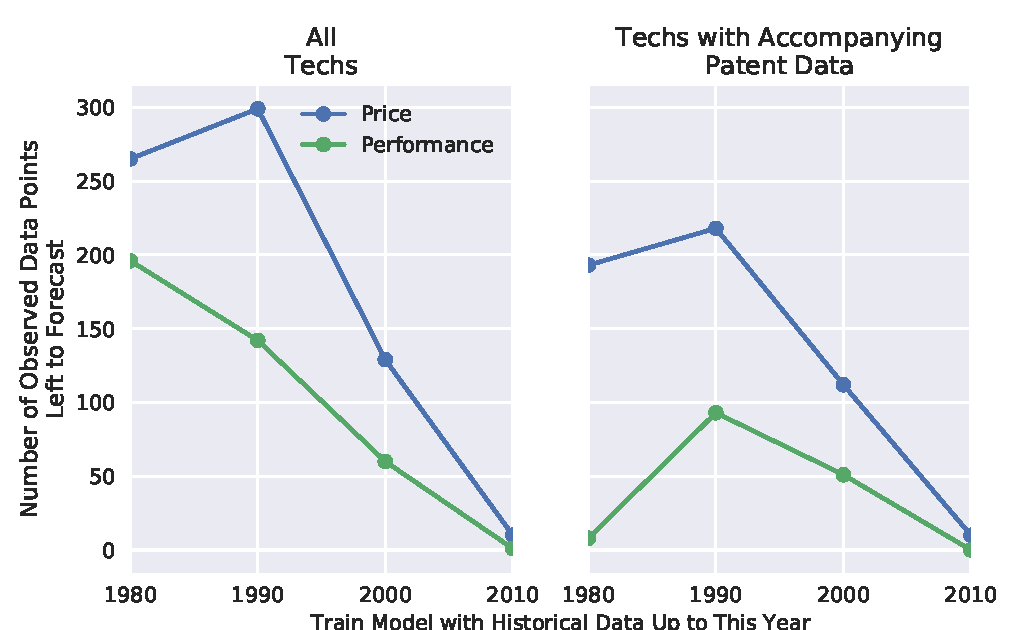
\includegraphics[width=.75\textwidth]{figs/Observed_Technology_Data_to_Forecast.pdf}
    \caption{\textbf{The number of data points available to forecast, given different training years.} Because the various technology trends started and stopped in different years, training in later years would allow more technologies to have had a trend. However, training in later years would leave fewer subsequent data points to forecast. In all conditions the observed data points were spread out across about 20 unique technologies. The training year used for this study was 1990.}
    \label{fig:Observed_Technology_Data_to_Forecast}
\end{figure}

Because we tested our forecasts on real historical data data, we needed some real historical data left to test with. In general, the later the date that we selected to train the models with, the less data we would have left to forecast and test on. However, this was not always the case. Because historical technology trends had a variety of start dates, we could only hope to train a model and make forecasts for those technologies that we had already ``seen," and so could only include those technologies for forecasting. We required that a technology trend needed 3 observed data points before we would train a model with it and make forecasts. Selecting a later training date, then, would allow more technologies to enter as candidates for forecasting. Thus, we have both a desire to push for earlier training dates to leave subsequent data for forecasting, and a desire to push for later training dates to allow more trends to be included for forecasting. Figure \ref{fig:Observed_Technology_Data_to_Forecast} shows the net effects of these two forces: the total number of data points that could be forecasted, given different training dates. In all cases, the observed data points are spread across about 20 technology trends. We selected 1990 as our training year to maximize the number of data points left to forecast and test the models. 

\begin{figure}
    \centering
    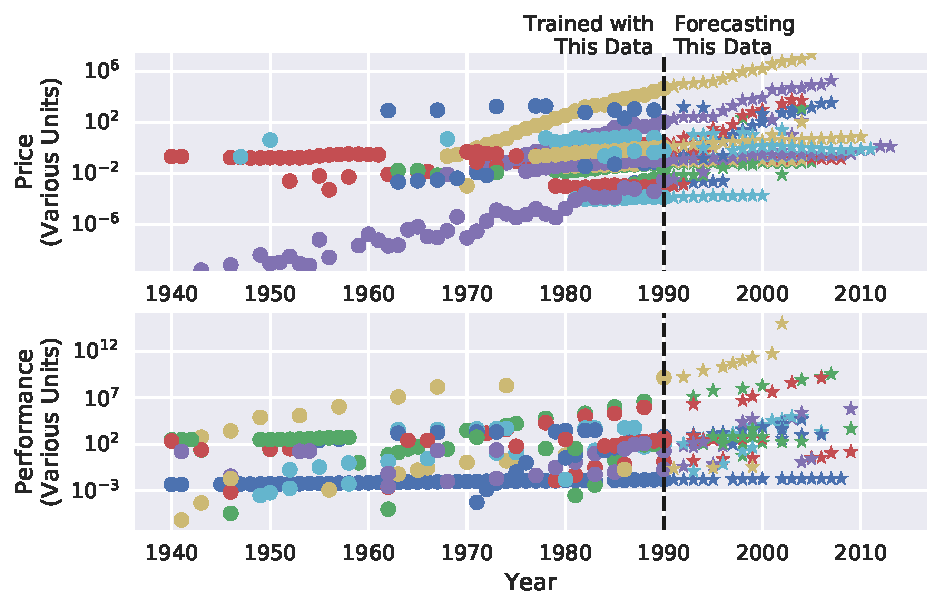
\includegraphics[width=.75\textwidth]{figs/Data_to_Forecast.pdf}
    \caption{\textbf{The technology data used to train and test the forecasting models.}}
    \label{fig:Data_to_Forecast_Performance}
\end{figure}

Figure \ref{fig:Data_to_Forecast_Performance} shows the final data that was used for training the models and for testing forecasts. When we tested adding patent data to improve forecasts, only a portion of this data was used, as only a portion of it had been connected to patent domains.

\section{Comparing Forecast Accuracy}

We began with perhaps the simplest possible trend extrapolation model, which we used as an example in section \ref{forecasting_basics}: ``every year the technology improves by a fixed amount, but each year there is some random noise around that improvement." The sizes of the fixed improvement and of the noise are the two parameters that the model must estimate from historical data and are what the models use to make forecasts. The previously shown Figure \ref{fig:forecast_evaluation} is an example forecast from this model, and all forecasts for all technologies are shown in section \ref{Each_Technology_Forecast}. 

\begin{figure}
    \centering
    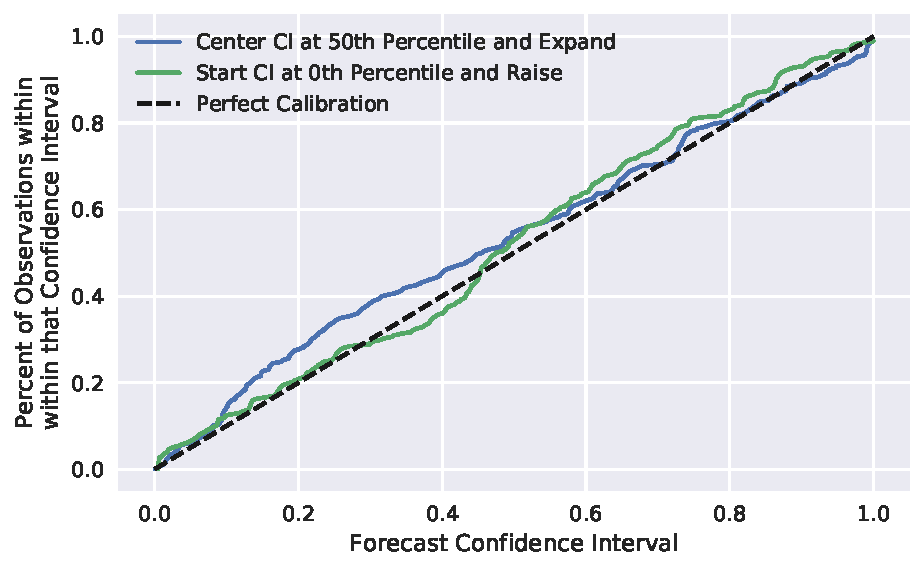
\includegraphics[width=.75\textwidth]{figs/Forecast_Calibration_Price.pdf}
    \caption{\textbf{Predictive models of technology price were well-calibrated.} For a perfectly-calibrated model, a forecast that a future data point will happen within a confidence interval of 95\% will later see data points falling within that range 95\% of the time. This is true for all confidence interval widths (dashed line). The predictive models of technology price closely followed this line using two different ways of defining the confidence interval. Blue line: centering the confidence interval at the median (50th percentile) predicted value and then expanding the width to incorporate higher and lower possible values. Green line: starting the confidence interval at the lowest (0th percentile) possible value and raising the confidence interval to consider larger possible values.}
    \label{Forecast_Calibration_Price}
\end{figure}

The models of price were well-calibrated (Fig. \ref{Forecast_Calibration_Price}). Of the 278 data points tested, the true data points occurred within the forecasts' 95\% confidence interval 94\% of the time, and within the 50\% confidence interval 55\% of the time. This is a marked advance in forecasting over simply drawing a line through the data points, as it means that we have statements of uncertainty about our forecasts that are explicit, quantitative, and (most usefully) rather close to true. Making forecasts that are correct about their uncertainty is useful, but it is even better if those forecasts can be more accurate; we want the same well-calibrated confidence intervals, but we want those confidence intervals to be tighter. We will return to this goal below.

\begin{figure}
    \centering
    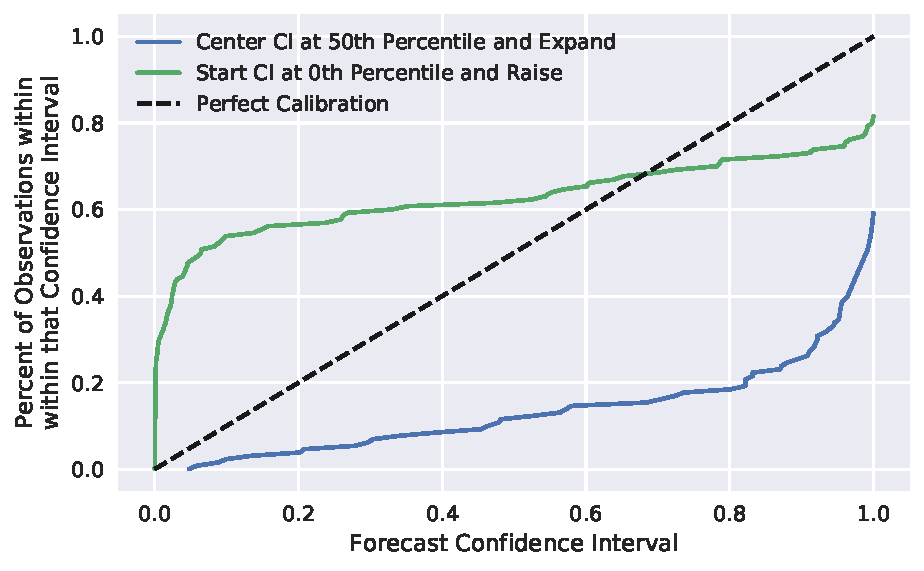
\includegraphics[width=.75\textwidth]{figs/Forecast_Calibration_Performance.pdf}
    \caption{\textbf{Predictive models of technology performance were terribly calibrated.} As Figure \ref{Forecast_Calibration_Price}, except for technology performance data.}
    \label{Forecast_Calibration_Performance}
\end{figure}

Unfortunately, the models of performance were poorly calibrated (Fig. \ref{Forecast_Calibration_Performance}). Of the 130 data points tested, the true data points occurred within the forecasts' 95\% confidence interval just 35\% of the time, and within the 50\% confidence interval just 12\% of the time. These mistakes show the models of performance are overconfident (their confidence intervals are too narrow). This fact is likely because the models are misspecified; they simply don't describe what's happening in the data well. Consider trying to use a straight line to model data that is actually a parabola (a U-shaped set of points). The model wouldn't describe the data well at all, and would yield terrible prediction. Better forecasts might be made with models that better describe the data.

In pursuit of more accurate forecasting, we trained 6 different kinds of more complex models and compared the accuracy of their forecasts to those of the simplest model described above. These models added additional complexity like ``the size of the improvement in this year depends somewhat on the size of the improvement last year," or even ``the size of the improvement in this year depends somewhat on the size of the improvement 5 years ago." Interestingly, these more complex models did not systematically raise the forecasting accuracy beyond the simplest model we started with (Figs.
\ref{fig:Separate_Models_Forecast_Quality_Price}, \ref{fig:Separate_Models_Forecast_Quality_Performance}). For each model some trends were forecasted slightly better, and others slightly worse, but the collective improvement was at best nil.

\subsection{Partial Pooling}\label{partial_pooling_section}
\begin{figure}
    \centering
    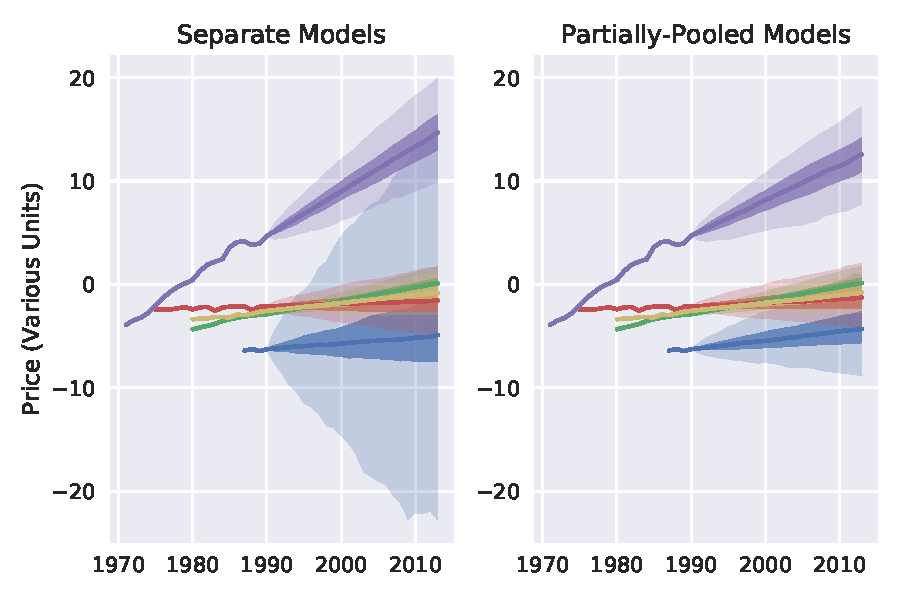
\includegraphics[width=.75\textwidth]{figs/Separate_vs_Pooled_Extrapolation_Demonstration_Price.pdf}
    \caption{\textbf{Combining inference of multiple technologies' trend extrapolation models can tighten forecasts.} Left) When modeling technologies separately, there was not much data for the price of natural gas-fired combined cycle gas turbines (blue). Accordingly, this left great uncertainty as to the year improvement rate or the variability around that rate, which led to very broad predictions. Right) By partially pooling the inference of all the technologies' trends, other technologies' behavior can inform our models of trends with little data. This allows for tighter forecasts.}
    \label{fig:Separate_vs_Pooled_Extrapolation_Demonstration}
\end{figure}

Another possible way to help statistical inference, and thus forecasting accuracy, is to recognize that each of these individual technology trends is not completely isolated. Instead, what we learn from one trend could help us when evaluating another. This could be particularly helpful if one technology doesn't have much data. We might not be able to very confidently infer what its yearly improvement rate is, but we might know from looking at other technologies what a \textit{typical} improvement rate is, and that can help inform our guess as to what this \textit{particular} technology's improvement rate is. Figure \ref{fig:Separate_vs_Pooled_Extrapolation_Demonstration} shows an example of this. On the left, we see data and forecasts for several technology trends, but one of them (blue) has very little data and so has great uncertainty in its forecasts (wide confidence intervals). On the right, we modify these models so that they assume that part of the information about each trend is unique to that trend but part is drawn from a shared pool of information that is true about all trends; this model structure is called ``partial pooling." Partial pooling can thus decrease our uncertainty for forecasts, and we see this on the right with the forecasts for the blue trend being much tighter.

\begin{figure}
    \centering
    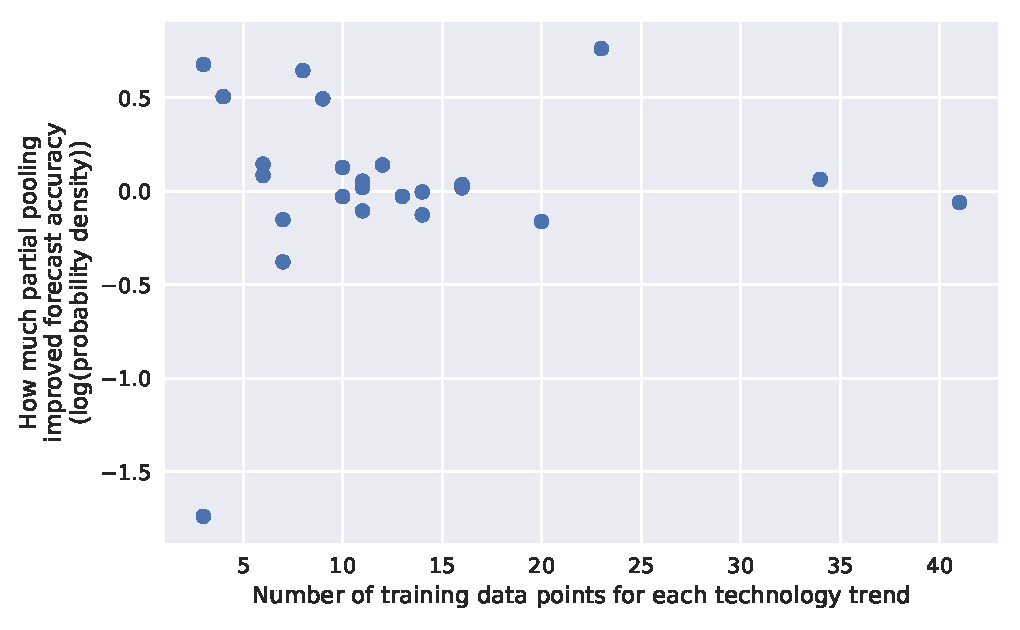
\includegraphics[width=.75\textwidth]{figs/Separate_vs_Pooled_Forecast_Accuracy_Price.pdf}
    \caption{\textbf{Partial pooling was mildly helpful for several technologies with less data, but hurt forecasting for one.} Trends visualized are for price data. The technology whose forecasts were notably hurt was hard drive prices (which had only 3 data points to train with).}
    \label{Separate_vs_Pooled_Forecast_Accuracy_Price}
\end{figure}

Partial pooling is not guaranteed to be helpful, because there's no guarantee that different trends are actually similar in any way. By using partial pooling, we're asserting that knowing something about how nuclear power improves should inform us about how hybrid corn improves. While this is likely true in a very general sense, if we read too much into how nuclear power improves, we may overapply that knowledge to hybrid corn and miss out on the properties that are different for corn. This happened when we used partial pooling to model price data. In general, partial pooling's effects on forecasts were either negligible or slight improvements, particularly for those technologies with little historical data to train on (Fig. \ref{Separate_vs_Pooled_Forecast_Accuracy_Price}). But the overapplication happened with hard drive prices, which had only 3 data points to train on. The model drew the wrong inferences from the other technologies and was overconfident in its predictions, making the forecasts worse. In aggregate, using partial pooling was not wildly helpful for price nor performance forecasting (Figs. \ref{fig:Pooled_Models_Forecast_Quality_Price} and \ref{fig:Pooled_Models_Forecast_Quality_Performance}).


\subsection{Adding Patent Data}
\begin{figure}
    \centering
    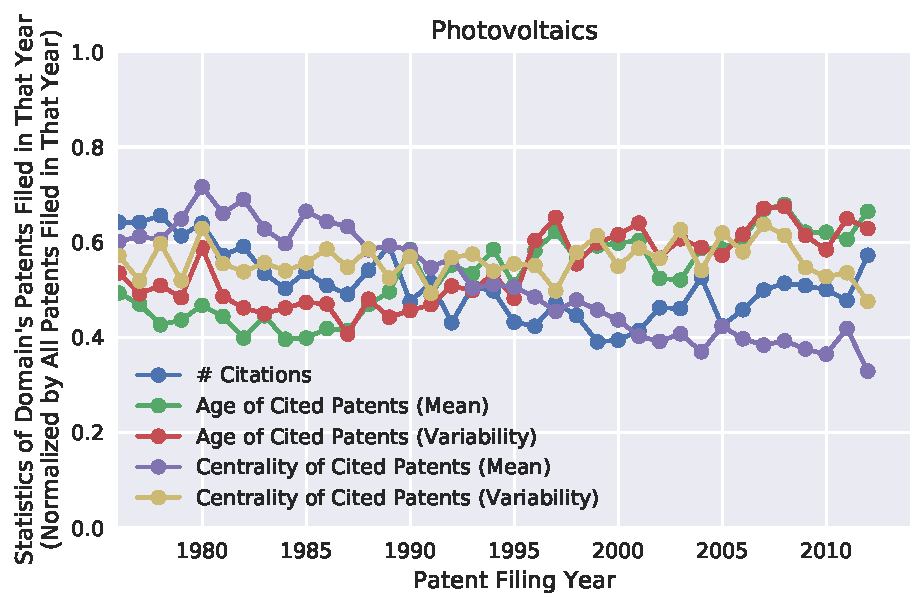
\includegraphics[width=.75\textwidth]{figs/Patent_Data_SOLAR_PV.pdf}
    \caption{\textbf{Several features of patents associated with photovoltaics, by patent filing year.} Each feature is expressed as a percentile score, compared to all patents in that filing year, and average across the patents relevant to photovoltaics. Data for other patent domains are shown in section \ref{patent_data}. These were the predictors used to attempt to improve technology forecasts.}
    \label{Patent_Data_Example}
\end{figure}

We tested if using information from patents could improve forecasts for those technology trends that had accompanying patent data. %Recall that these technology trends were said to be in a domain (e.g. hard drives were in ``magnetic information storage" and DNA sequencing was in ``genomics"), and then a set of patents were identified as belonging to each of those domains. P
Patents are rich with metadata, such as the citations they make to other patents. These metadata can be used to calculate multitudes of properties of patents, but these five have been previously found to either correlate with technology improvement rates or patent quality:

\begin{itemize}
    \item the number of citations the patents made
    \item the average age of the patents' cited patents
    \item the variability of the age of the patents' cited patents
    \item the average centrality\footnote{The centrality of a patent is how central it is in the \textit{entire} patent citation network, incorporating all observed years of data. It is a measure of how many other patents are reachable from the target patent by going through its citations, then through its cited patents citations, and so on.} of the patents' cited patents
    \item the variability of the centrality of the patents' cited patents
\end{itemize}

An example of these data for the domain of photovoltaics is shown in Figure \ref{Patent_Data_Example}, and figures for all domains are in section \ref{patent_data}. The method for calculating these predictors was as follows: First, the candidate predictors were calculated for each individual patent. Then, each patent's predictor values were compared to the values of all patents filed in the same year, then expressed as a percentile. Finally, the normalized predictor values for all patents in a domain were averaged together, for each filing year. This year-by-year, normalized predictor data  was the data used to try to improve technology performance and price forecasting. Because patent data was only available from 1975 onward, these models were only trained with patent and technology data from 1975 onward (up to 1990, for a total of 15 years of possible data).

Again, the simplest model was ``every year the technology improves by a fixed amount, but each year there is some random noise around that improvement." We added patent data to this by adding ``the patent predictor from a previous year may also have some influence." Unfortunately, not one of the patent predictors systematically improved forecasting above the simplest model (Figs. \ref{fig:VAR_Model_Prediction_increase_Price}, \ref{fig:VAR_Model_Prediction_increase_Performance}).  We tried adding influence from just the immediately previous year, 5 years previous, or both, but none of these modifications markedly altered the forecasting accuracy of the models (Figs. \ref{VAR_Model_Prediction_Citations_Backward_N_Price}-\ref{VAR_Model_Prediction_stdSPNPcited_1year_before_Performance}).

\begin{figure}
    \centering
    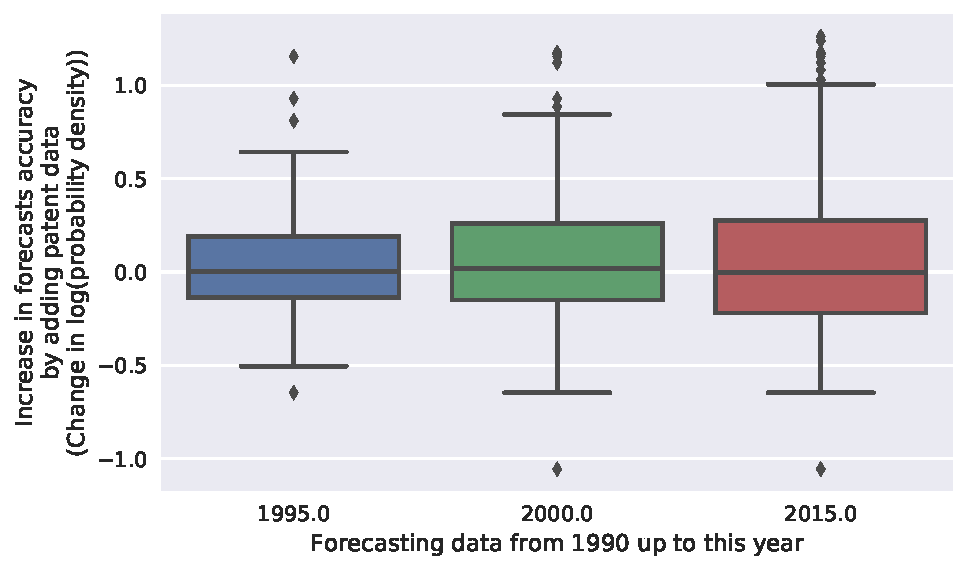
\includegraphics[width=.75\textwidth]{figs/VAR_Model_Prediction_increase_Price.pdf}
    \caption{\textbf{Adding patent data did not improve forecasts of technology price.} Box plots: The difference in all forecasted data point's log(probability density) after adding patent data to the model vs. not including patent data. Regardless of whether one considers just data that was 5 years into the future (blue), 10 years (green) or all possible data (red), the forecasts were not consistently better. This visualization shows the results for using only one predictor: the average centrality of the patents cited. However, the forecasting accuracies are qualitatively similar with other predictors (see Figs. \ref{VAR_Model_Prediction_Citations_Backward_N_Price}-\ref{VAR_Model_Prediction_stdSPNPcited_1year_before_Performance}).}
    \label{fig:VAR_Model_Prediction_increase_Price}
\end{figure}

\begin{figure}
    \centering
    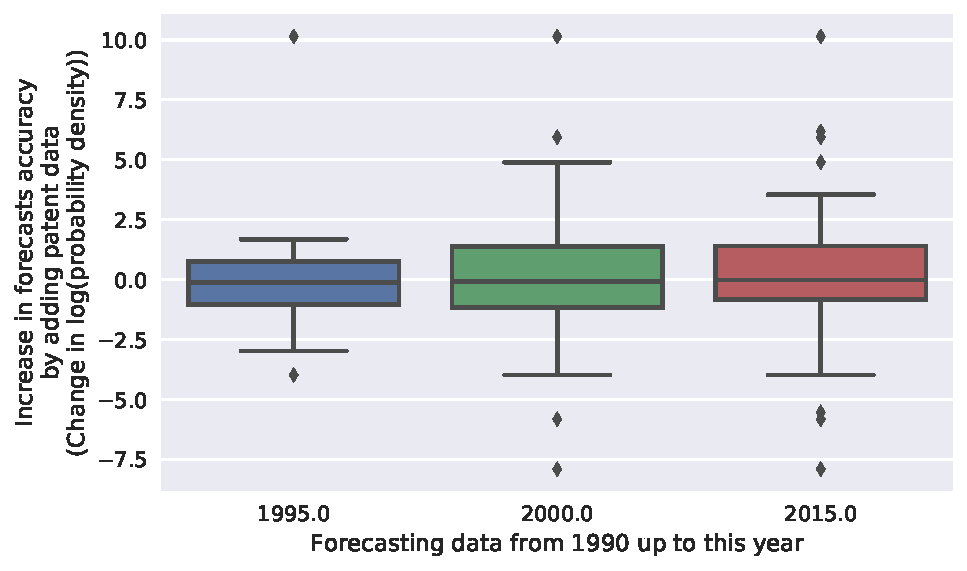
\includegraphics[width=.75\textwidth]{figs/VAR_Model_Prediction_increase_Performance.pdf}
    \caption{\textbf{Adding patent data did not improve forecasts of technology performance.} As Figure \ref{fig:VAR_Model_Prediction_increase_Price}, but for technology performance trends instead of price trends.}
    \label{fig:VAR_Model_Prediction_increase_Performance}
\end{figure}

\section{What Went Right, What Went Wrong}
About half of the tasks went right and about half went wrong. ``Right" here means that we produced a forecasting system that does the desired task well. ``Wrong" here means that we produced results that went counter to a hypothesis. However, both positive and negative results are still results, and both can be learned from. 

\subsection{Price was well-specified, while Performance was not}
Forecasting of price data worked very well, in that well-calibrated forecasts were made across many disparate technologies. Previous research\footcite{Farmer2016} pioneered using the same trend extrapolation methods on part of this data, but using non-Bayesian methods. Those methods produced confidence intervals that were less well-calibrated than the forecasts of the present study, and that is likely due to an advantage of Bayesian prediction: uncertainty in our parameters. The forecasts here took into account our uncertainty in the models' parameters, and so had wider confidence intervals.\footnote{Put technically: The forecasted data points were modeled as normally-distributed random variables. In a Bayesian framework, estimating a normally-distributed random variable with a scale that is also an inferred parameter yields a posterior distribution that has heavier-than-normal tails. In a frequentist framework the scale is just taken as the best-fit value, and the forecasts are normally distributed.} Interestingly, that previous research used slightly more complicated models to fit the data, but here we find that they conferred no advantage in forecasting accuracy.

Forecasting of performance data, however, was rubbish. Some of this could be due to prosaic reasons: there was less performance data than price data, there were more gaps with missing years of data than the price data, and much of the data came from a pieced-together collection that may have been more prone to errors. But that shouldn't have led to forecasting this bad. Instead, what was probably most important is that the models were misspecified. 

One obvious way that the models were misspecified is that this data is clearly more of a sequence of rough steps than a smooth progression. The models we created didn't allow for the possibility of long periods of no improvement, followed by a jump. This led the real data to be persistently lagging under or leaping over the models' forecasts, which creates the terrible prediction. It's worth noting that the \textit{reality} may not have such rough steps. With more complete sampling, the year-by-year changes in artifact performance would still be steps but could be more smooth. However, what we are trying to model here is not just the performance of artifacts in the world, but also the rate at which observations are recorded into our data set. Adding a simple step function into the models would not be difficult and is low-hanging fruit for making improvements. There is, however, a wide world of more complex models for record-breakers\footcite{Berdahl2017}; testing this wider set of models would be a more substantive project.

\subsection{Patents: \textit{This} data is not a predictor}
Using patent data to improve technology forecasting was a task that, if it had succeeded, would have been a huge advance. For years it has been an open research question as to how to match up technologies (artifacts that people are using) with patents (legal documents filed to protect property rights on a particular way of doing things). While in principle any given product may employ techniques that the producing company has patented, in practice companies do not advertise or even record virtually any of those patent-product pairings. What's more, precise patent-product matching is often not the right description of reality. Instead, there is a cluster of patents created by an ecosystem of inventors that contains the collective knowledge of an area of technology, and this ecosystem sometimes also yields quantifiably better artifacts. How to identify such ecosystems of patents has been an area of active research. 

This study used patents that were previously identified with the specific aim of matching them to historical performance and price data.\footcite{Benson2012,Benson2014} That line of research found that these patents had citation-based features that correlated strongly with technology's average improvement rates.\footcite{Benson2015,Triulzi2017} However, this data has not borne more accurate forecasts than trend extrapolation alone.\footnote{If one does not have data for a historical trend, then this particular patent data may still be useful for making estimates of which technologies are improving faster. These researchers are pursuing exactly this strategy: \cite{Benson2016}}

Because matching patents and artifacts is so complex, the current results are not a definitive conclusion that patents cannot be used to improve technology forecasts. There are many ways in which the methods could be revised, including how technologies are matched with patent domains (e.g. perhaps they are a weighted sum of multiple domains) and how patent domains are defined (e.g. natural language processing may better extract important developments from patents than citation data). Given continued advances in large-scale data collection and processing, it's a reasonable prediction that technical data like patents will eventually be used to make forecasts that are more accurate than simple trend extrapolation.

\newpage
% \newrefsection

% \title{Appendix}
% \maketitle
\beginsupplement

\section*{Appendix}

\addcontentsline{toc}{section}{Appendix}


\section{Technology Data and Forecasts}
\subsection{Metadata on Historical Trends}\label{time_series_metadata}
The following pages include metadata on the technology trend data used in this study. The data were collected by contacting the authors of the original journal articles in which these data were published, and the metadata are reproduced nearly exactly as they were received from the researchers. As such, they are rough and require interpretation, which is exactly the point: we did not want to overinterpret the data by simplifying or polishing it. The only modification to the data is that the data from the Farmer \& Lafond paper is of the form ``lower is better," with units to match. For this study we simply inverted that data so ``higher is better," and thus the units are the reverse of those shown here. 

Some data were identified as questionable, for reasons given previously, and are labeled as such here. Those data were not used in this study.

\newgeometry{margin=.1in} % modify this if you need even more space
\begin{landscape}
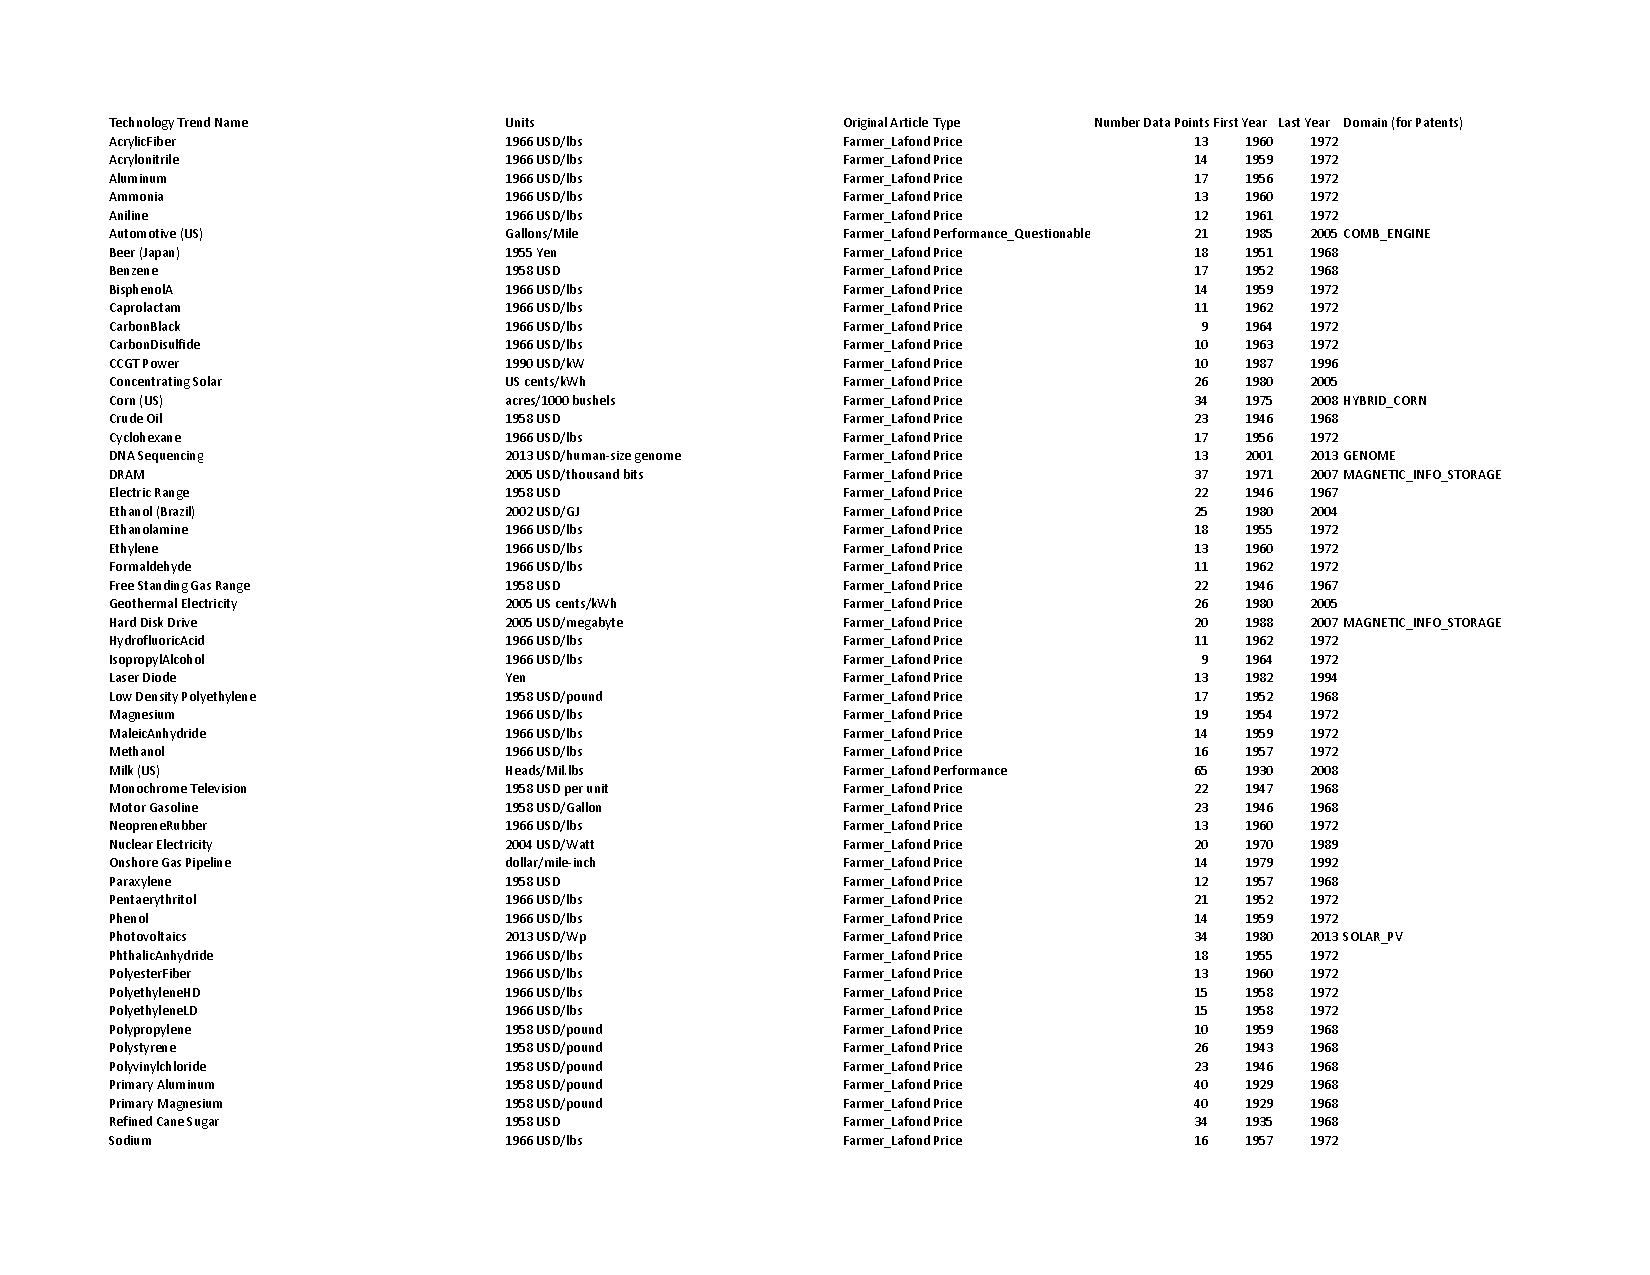
\includepdf[pages=-]{figs/time_series_metadata.pdf}
\end{landscape}
\restoregeometry

\subsection{All Technology Forecasts}\label{Each_Technology_Forecast}
The following pages show the trends and forecasts for all technologies in the study (first price trends, then performance trends). Note that in price trends the technology can get both better and worse, and so the forecasts reflect this, while in performance trends the technology is defined as only able to improve with time, and so the forecasts reflect that. Additionally, some of these technology trends had missing data (i.e. years in which there were no observed or recorded data points). The software developed for this study automatically makes estimates on what the missing data was, just as it does for the forecasts (which is just ``missing" future data!). Such missing data could include data before the data point; there's no mathematical difference between making forecasts into the future vs. backcasts into the past, and so these are automatically generated by the software.

As described in the previous section, the technology names and units are shown exactly as they were received from the original researchers. Note that, as described previously, for the data from Farmer \& Lafond the units are of the form ``lower is better," and so to match with the rest of the data these were inverted. Thus the units are the reverse of those shown for these graphs.

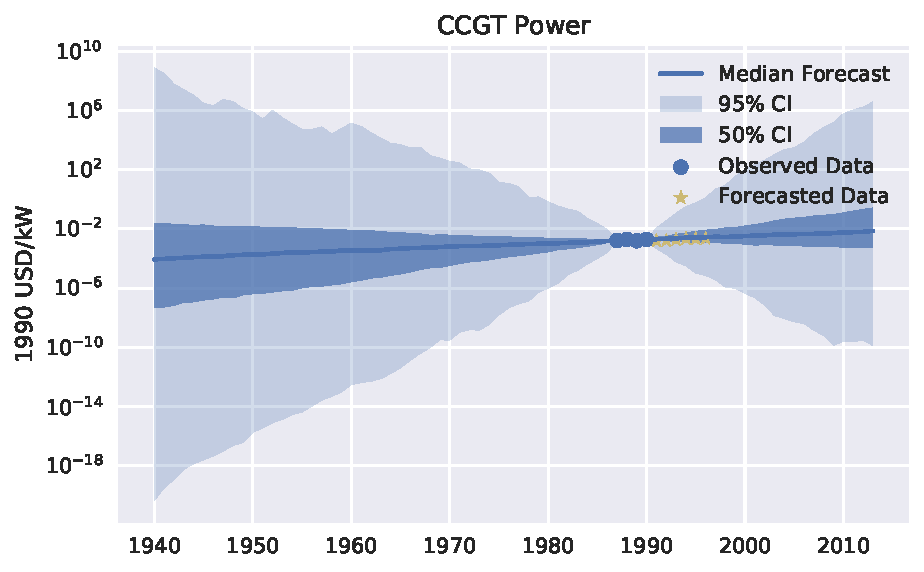
\includepdf[pages=-]{figs/Each_Technology_Forecast.pdf}

\subsection{All Patent Domains}\label{patent_data}
These candidate predictors were calculated for each filing year for all patents filed in that year and expressed as a percentile, relative to the other patents in that filing year. Then for each domain the value of that predictor for each year was taken to be the average of the domain's patents filed in that year. This was the data used to try to improve technology performance and price forecasting. Because patent data was only available from 1975 onward, these models were only trained with patent and technology data from 1975 onward (up to 1990, for a total of 15 years of possible data).

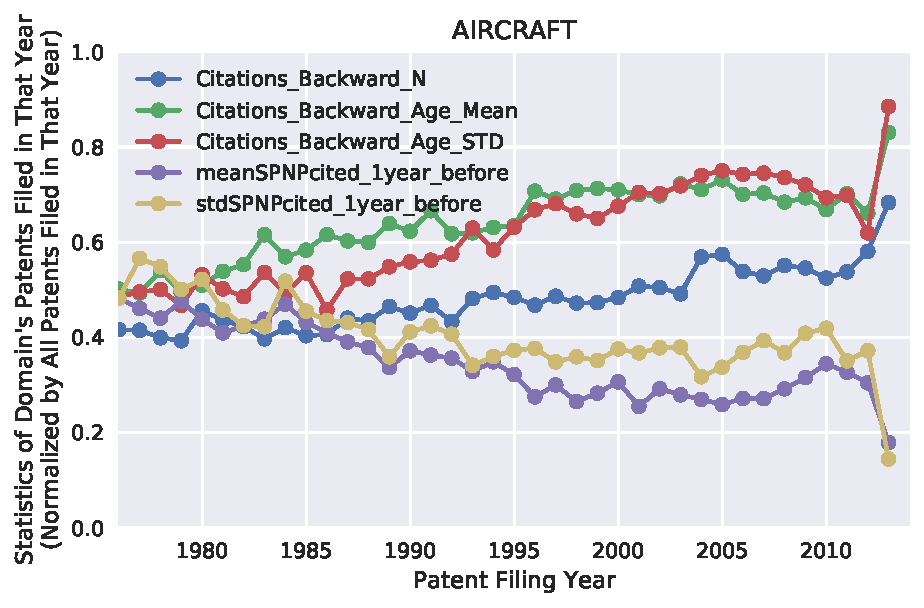
\includepdf[pages=-]{figs/patent_data_plots.pdf}

\section{Technical Materials}
\subsection{Mathematical Models}
\subsubsection{ARIMA}
The time series models were all modifications of ARIMA models (AutoRegressive Integrative Moving Average). The Integrative aspect says that instead of trying to model the level of a time series ($Y$) at year $t$ ($Y_t$) we are modeling its change from the previous year ($Y_t-Y_{t-1}$). The simple model of a fixed improvement every year with noise is:

$Y_t-Y_{t-1} \sim \mu + \epsilon_t$

$\epsilon_t \sim normal(0, \sigma)$

and we have prior beliefs on these parameters of:

$\mu \sim normal(0,4)$

$\sigma \sim cauchy(0,4)$

The basic ARIMA model can be expanded by adding a Autoregressive element, which says the percent change in the previous year also contributes:

$Y_t-Y_{t-1} \sim \mu + \epsilon_t + \phi (Y_{t-1}-Y_{t-2})$

with a prior of

$\phi \sim normal(0,4)$

This can be expanded to multiple steps backward in time, or to specific years. Here is what we term an ARIMA([1,5], 0) model\footnote{Typical nomenclature would denotes an ARIMA model by ARIMA($p,d,q$), with $p$ the number of AR elements, $d$ the number of differencing used, and $q$ the number of MA elements. Since all the models used in the present study are $d=1$ we drop them from the notation, and we go in more detail for $p$ and $q$ as to which exact lags are being used for the AR and MA elements}:

$Y_t-Y_{t-1} \sim \mu + \epsilon_t + \phi_1 (Y_{t-1}-Y_{t-2}) + \phi_5 (Y_{t-5}-Y_{t-6})$


The basic ARIMA model can also be expanded by adding a Moving Average element, which says the noise in the previous year also contributes:

$Y_t-Y_{t-1} \sim \mu + \epsilon_t + \theta \epsilon_{t-1}$

with a prior of

$\theta \sim normal(0,4)$

This can be also expanded to multiple steps backward in time, or to specific years. Here is what we term an ARIMA(0, [1,5]) model:

$Y_t-Y_{t-1} \sim \mu + \epsilon_t + \theta_1 \epsilon_{t-1} + \theta_5 \epsilon_{t-5}$

The Autoregressive and Moving Average elements can be combined, such as in this ARIMA([1,5], [1,5]) model:

$Y_t-Y_{t-1} \sim \mu + \epsilon_t + \phi_1 (Y_{t-1}-Y_{t-2}) + \phi_5 (Y_{t-5}-Y_{t-6}) + \theta_1 \epsilon_{t-1} + \theta_5 \epsilon_{t-5}$

For performance data, a constraint was added that the change ($Y_t-Y_{t-1}$) could only be positive. 

These were the models used in Figures \ref{fig:Separate_Models_Forecast_Quality_Price} and \ref{fig:Separate_Models_Forecast_Quality_Performance}.

\begin{figure}
    \centering
    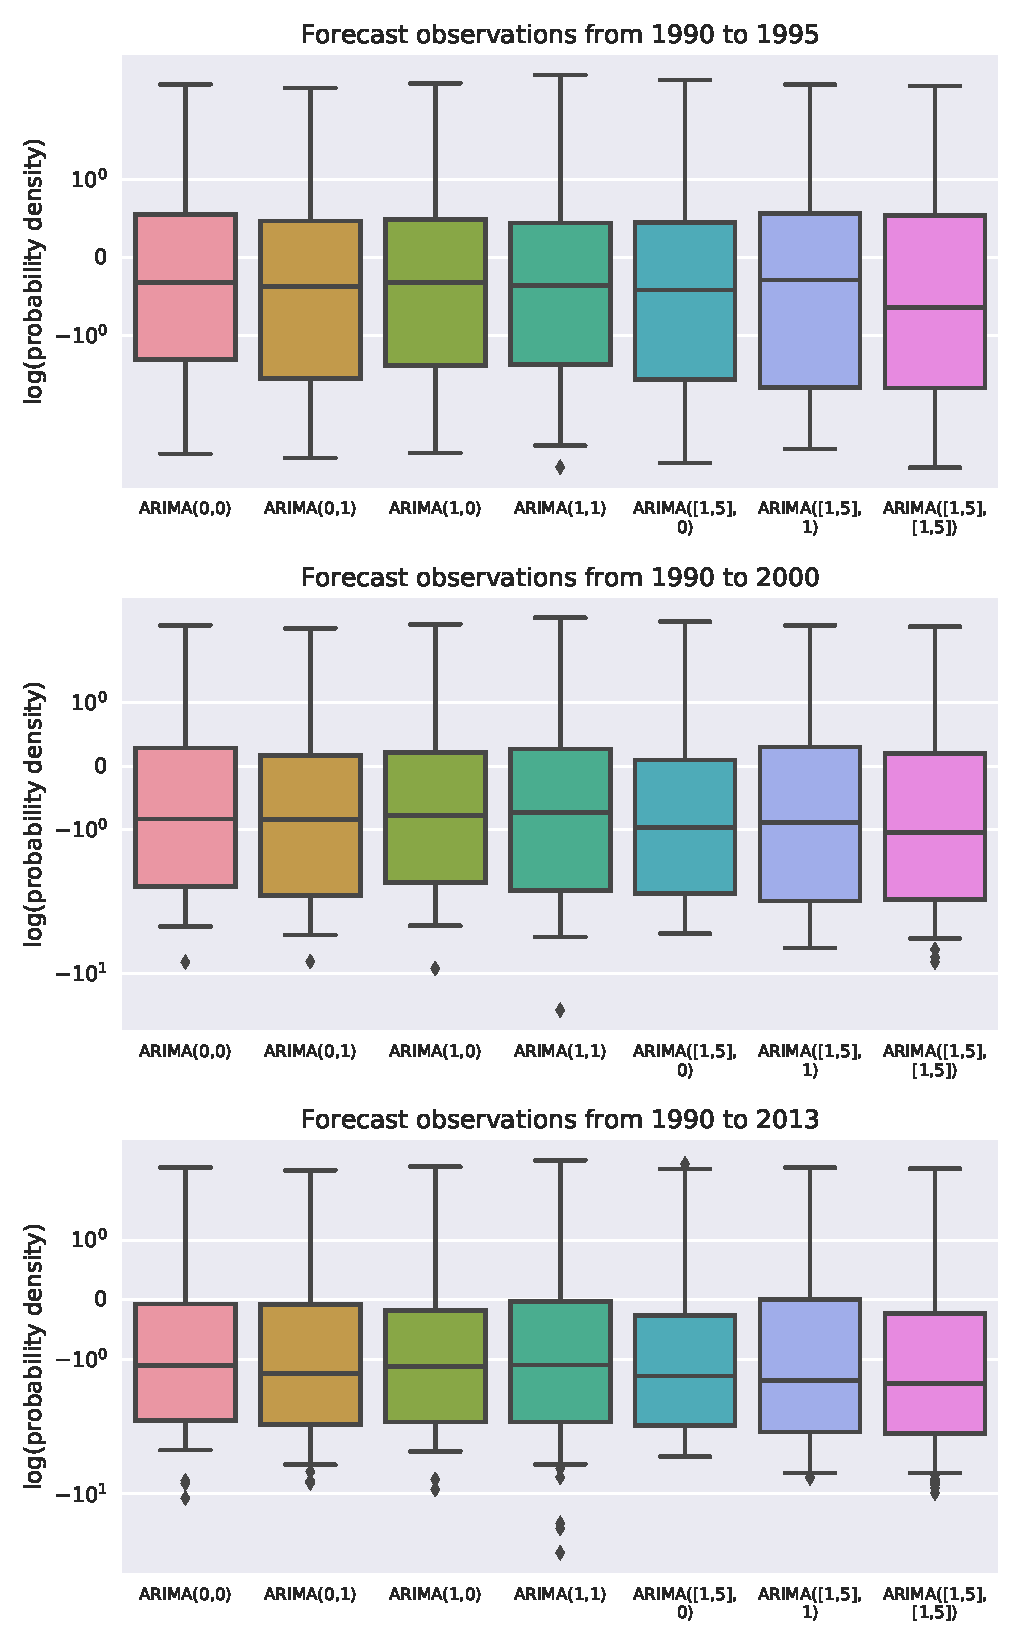
\includegraphics[height=.75\textheight]{figs/Separate_Models_Forecast_Quality_Price.pdf}
    \caption{\textbf{Distribution of forecasts' accuracies for different models of technology price.}}
    \label{fig:Separate_Models_Forecast_Quality_Price}
\end{figure}

\begin{figure}
    \centering
    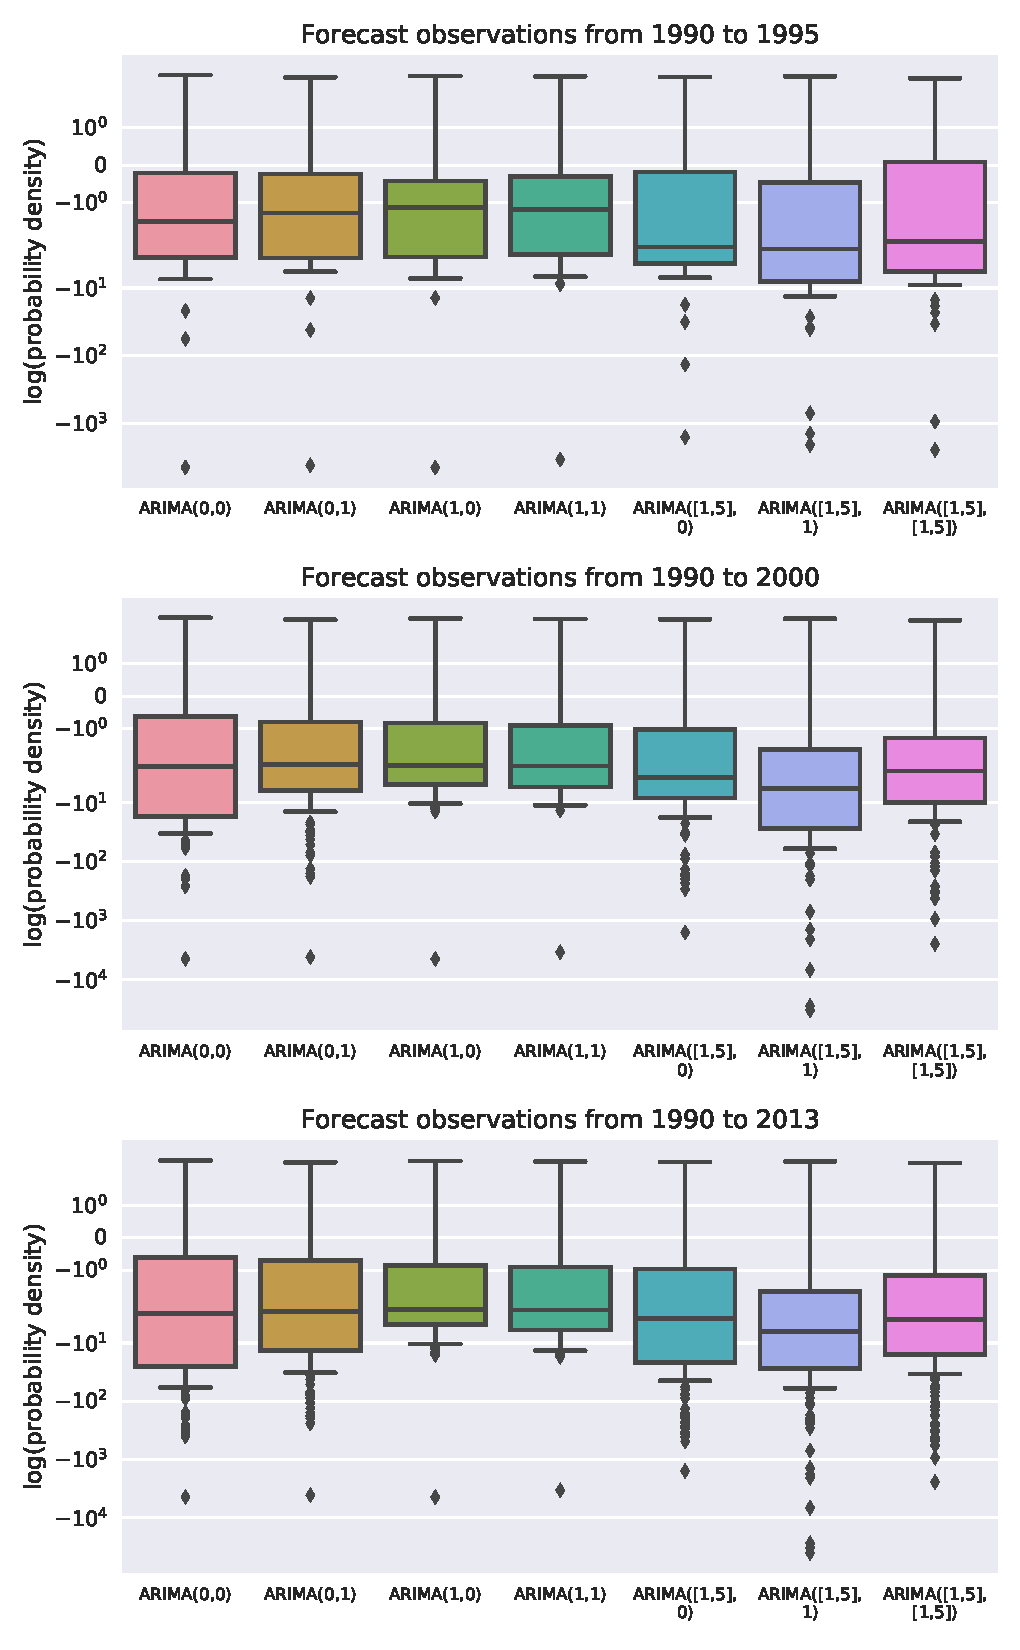
\includegraphics[height=.75\textheight]{figs/Separate_Models_Forecast_Quality_Performance.pdf}
    \caption{\textbf{Distribution of forecasts' accuracies for different models of technology performance.}}
    \label{fig:Separate_Models_Forecast_Quality_Performance}
\end{figure}

\subsubsection{Partial Pooling}
In partial pooling, the overall model structure is the same, but the parameter values for each individual trend $Y_{i}$ are collectively drawn from a multinormal distribution:

$Y_{i,t}-Y_{i,t-1} \sim \mu_i + \epsilon_t$

$\epsilon_t \sim normal(0, \sigma_i)$

$[\mu_i, \sigma_i] \sim [\hat{\mu}, \hat{\sigma}] + multinormal(0,diag(\tau)*\Omega*diag(\tau))$

Priors:

$\hat{\mu} \sim normal(0,4)$

$\hat{\sigma} \sim cauchy(0,4)$

$\tau \sim cauchy(0,1)$ (How much each parameter varies across the time series)

$\Omega \sim LKJ(1)$ (How the parameters correlate with each other across the time series)

This could be extended to the various kinds of ARIMA models by adding Autoregressive or Moving Average elements, and this was done for the models shown in Figures \ref{fig:Pooled_Models_Forecast_Quality_Price} and \ref{fig:Pooled_Models_Forecast_Quality_Performance}.

\begin{figure}
    \centering
    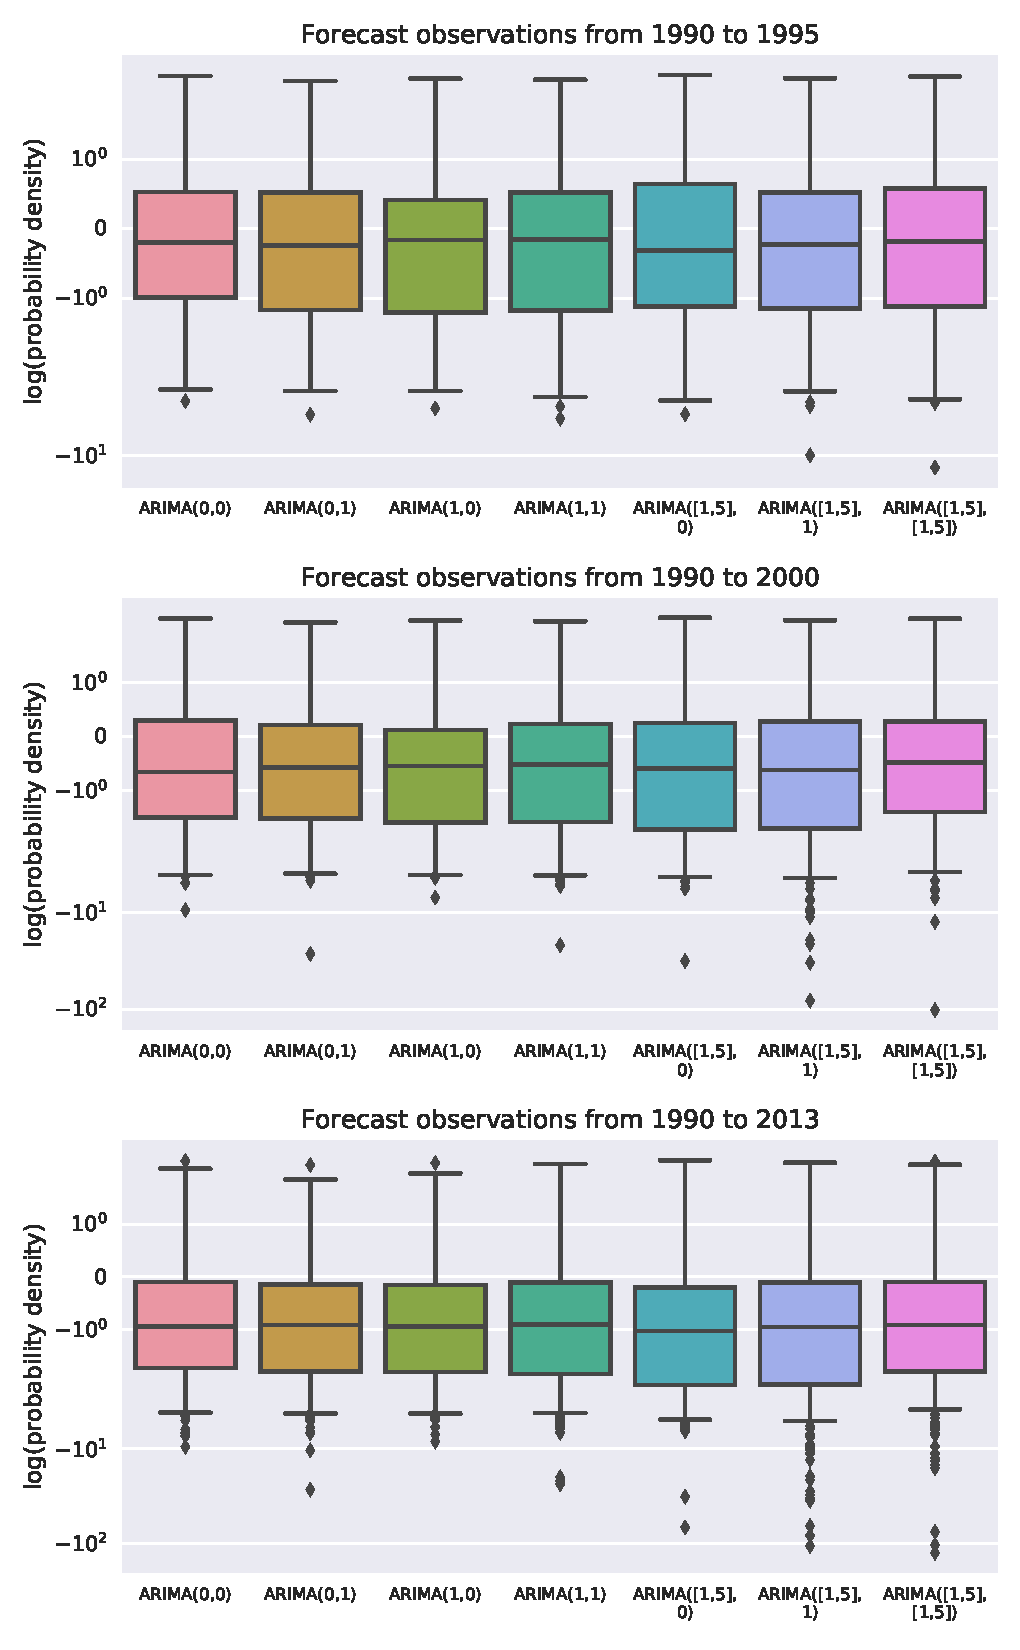
\includegraphics[height=.75\textheight]{figs/Pooled_Models_Forecast_Quality_Price.pdf}
    \caption{\textbf{Distribution of forecasts' accuracies for different models of technology price, using partial pooling.}}\label{fig:Pooled_Models_Forecast_Quality_Price}
\end{figure}

\begin{figure}
    \centering
    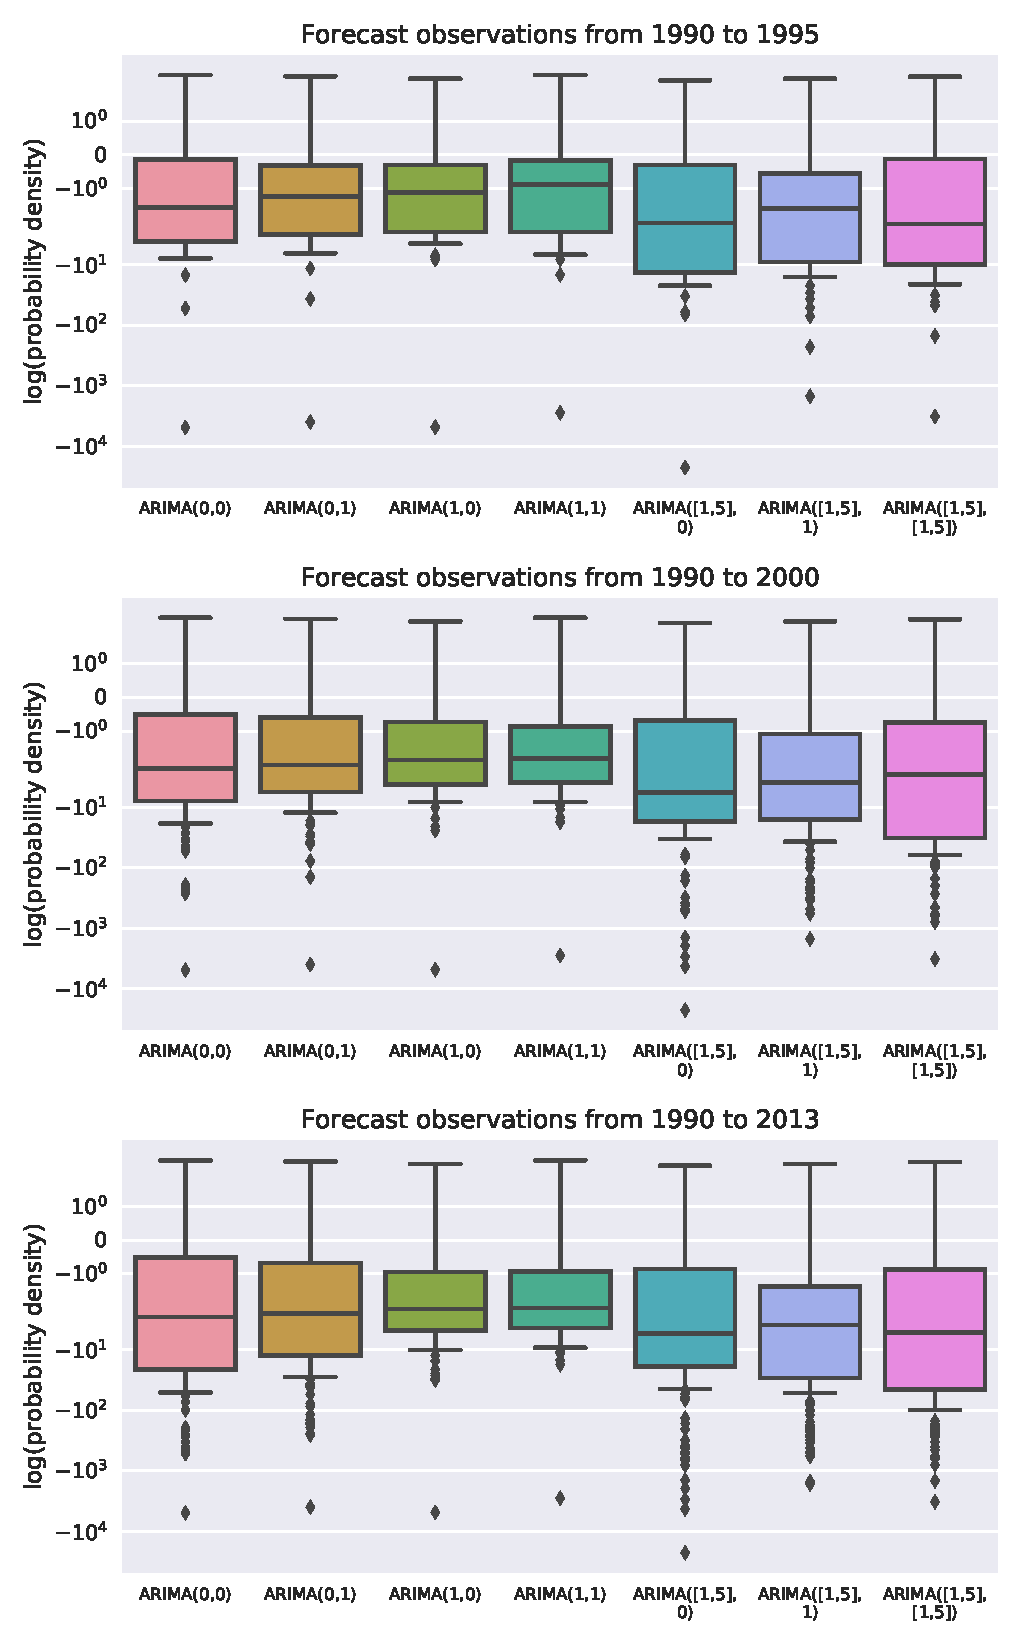
\includegraphics[height=.75\textheight]{figs/Pooled_Models_Forecast_Quality_Performance.pdf}
    \caption{\textbf{Distribution of forecasts' accuracies for different models of technology performance, using partial pooling.}}\label{fig:Pooled_Models_Forecast_Quality_Performance}
\end{figure}

\subsubsection{Vectorizing}
For adding in patent data, a multidimensional or vectorized version of the models were used. Each trend is actually a vector with $D$ dimensions, and those different dimensions could affect each other with some lag:

$\vec{Y}_{t} = [Y_{1,t}, Y_{2,t}, Y_{3,t}...Y_{D,t}]$ 

$\vec{Y}_{t} - \vec{Y}_{t-1} \sim \vec{\mu} + \vec{\epsilon}_{t} + \mathbf{P}(\vec{Y}_{t-1}-\vec{Y}_{t-2})$

$\vec{\epsilon}_t \sim normal(0, \vec{\sigma})$

where $\mathbf{P}$ is a $D x D$ matrix


Priors (for each element in the vector or matrix):

$\vec{\mu} \sim normal(0,4)$

$\vec{\sigma} \sim cauchy(0,4)$

$\mathbf{P} \sim normal(0,4)$

This could be extended by adding Moving Average elements, or even partially pooled. 

In this study, a different model was created for each of the candidate predictors created from the patent data (e.g. number of citations). One dimension of $\vec{Y}$ was the patent predictor, and the other was either price or performance. It would also be possible to put all the predictors together with both price and performance into a single, large $\vec{Y}$, but this would take much longer to run, and the negative results from the simpler models didn't indicate there was any signal from this patent data. 

This style of model is commonly called a VAR (Vector AutoRegression) model, though typically the errors of the different dimensions are correlated by being drawn collectively from a multinormal:

$\vec{\epsilon}_t \sim multinormal(0,diag(\tau)*\Omega*diag(\tau))$

This would be particularly appropriate if in the system being modeled noise/shocks from one dimension could affect another dimension at a timescale faster than that being sampled (i.e. faster than the time difference between $t$ and $t_1$). That did not seem likely in for the technology trend data in the current study, and so we left the errors uncorrelated. 

\newpage
\begin{figure}
    \centering
    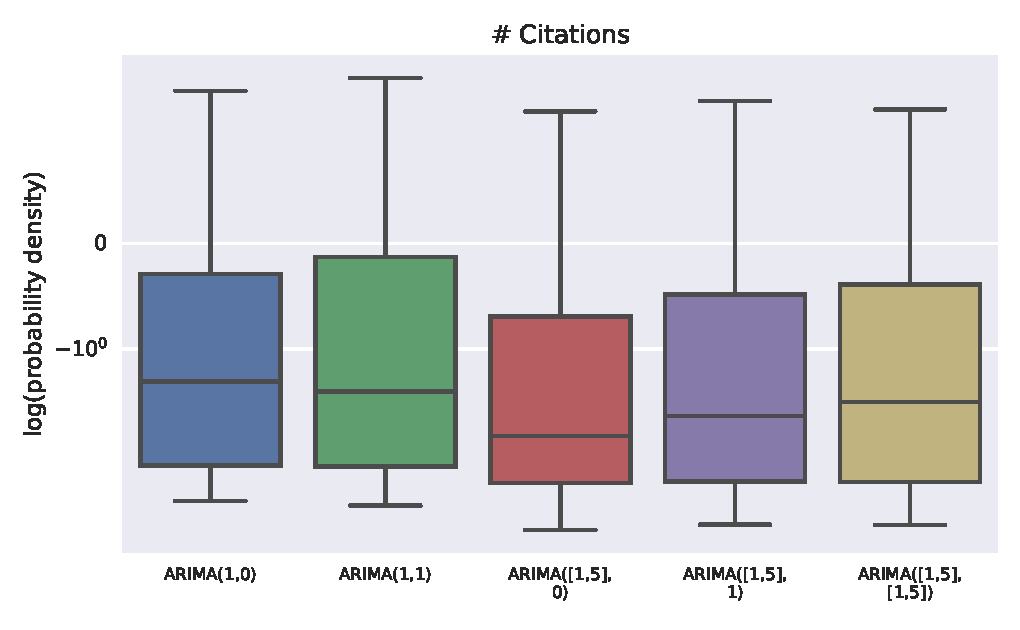
\includegraphics[width=.75\textwidth]{figs/VAR_Model_Prediction_Citations_Backward_N_Price.pdf}
    \caption{\textbf{Distribution of forecasts' accuracies for different models of technology price, using associated patents' number of citations.}}
    \label{VAR_Model_Prediction_Citations_Backward_N_Price}
\end{figure}

\begin{figure}
    \centering
    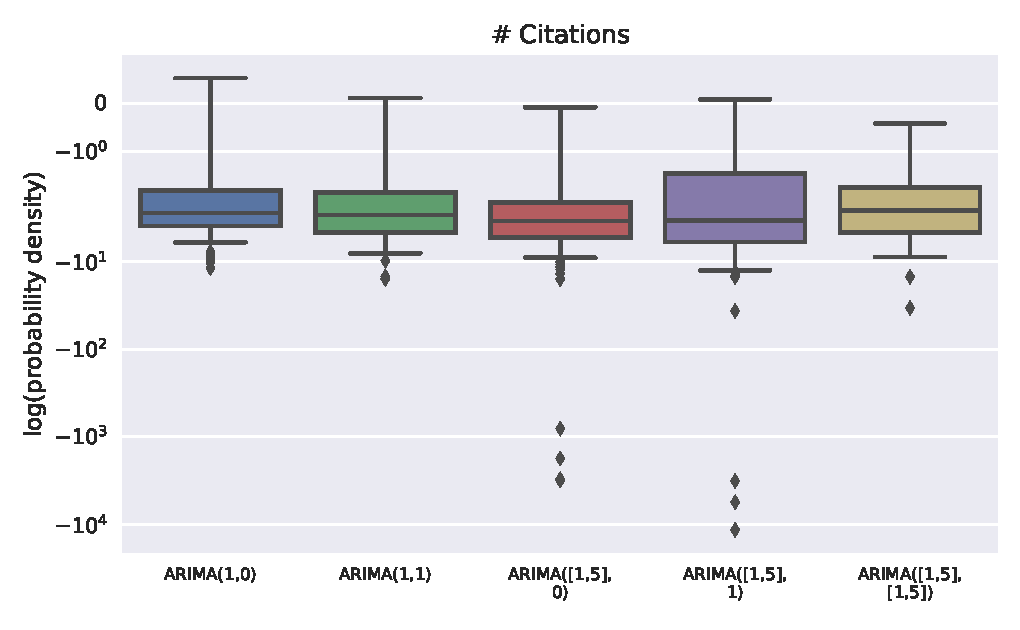
\includegraphics[width=.75\textwidth]{figs/VAR_Model_Prediction_Citations_Backward_N_Performance.pdf}
    \caption{\textbf{Distribution of forecasts' accuracies for different models of technology performance, using associated patents' number of citations.}}
    \label{VAR_Model_Prediction_Citations_Backward_N_Performance}
\end{figure}

\begin{figure}
    \centering
    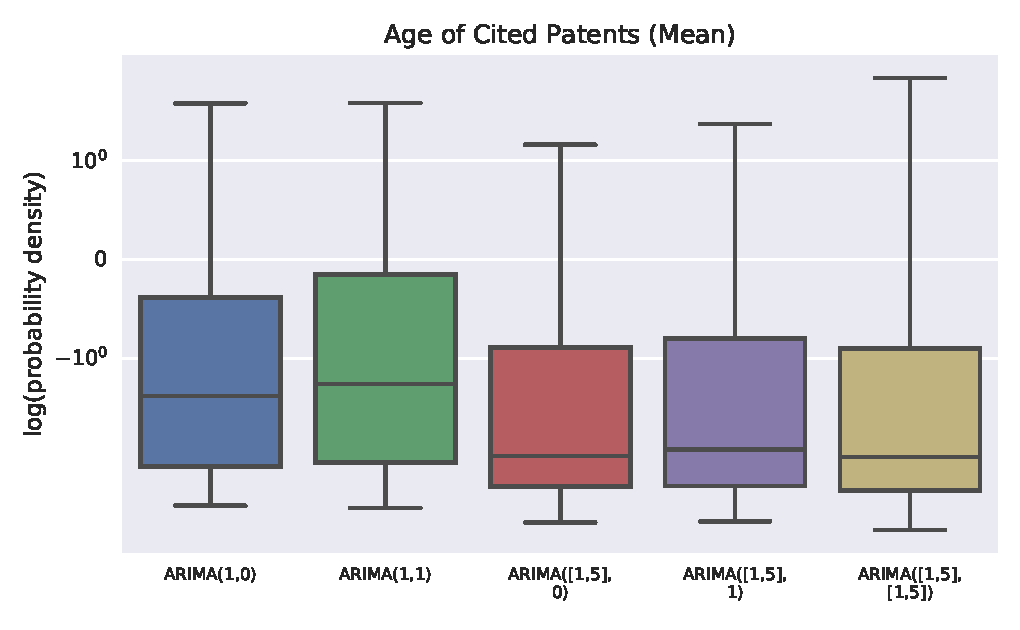
\includegraphics[width=.75\textwidth]{figs/VAR_Model_Prediction_Citations_Backward_Age_Mean_Price.pdf}
    \caption{\textbf{Distribution of forecasts' accuracies for different models of technology price, using associated patents' mean age of cited patents.}}
    \label{VAR_Model_Prediction_Citations_Backward_Age_Mean_Price}
\end{figure}

\begin{figure}
    \centering
    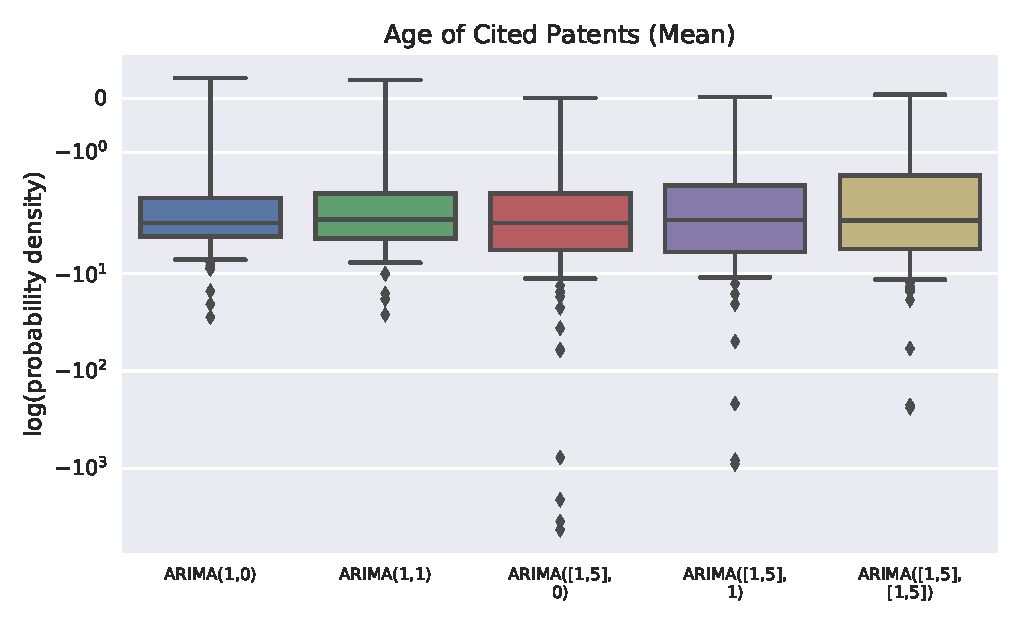
\includegraphics[width=.75\textwidth]{figs/VAR_Model_Prediction_Citations_Backward_Age_Mean_Performance.pdf}
    \caption{\textbf{Distribution of forecasts' accuracies for different models of technology performance, using associated patents' mean age of cited patents.}}
    \label{VAR_Model_Prediction_Citations_Backward_Age_Mean_Performance}
\end{figure}

\begin{figure}
    \centering
    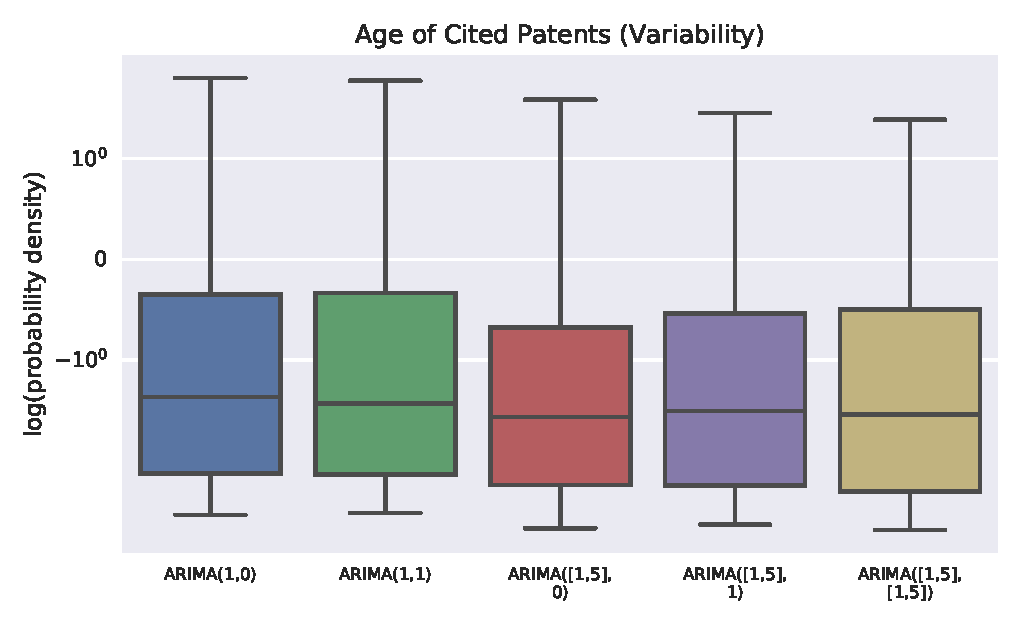
\includegraphics[width=.75\textwidth]{figs/VAR_Model_Prediction_Citations_Backward_Age_STD_Price.pdf}
    \caption{\textbf{Distribution of forecasts' accuracies for different models of technology price, using associated patents' variability of age of cited patents.}}
    \label{VAR_Model_Prediction_Citations_Backward_Age_STD_Price}
\end{figure}

\begin{figure}
    \centering
    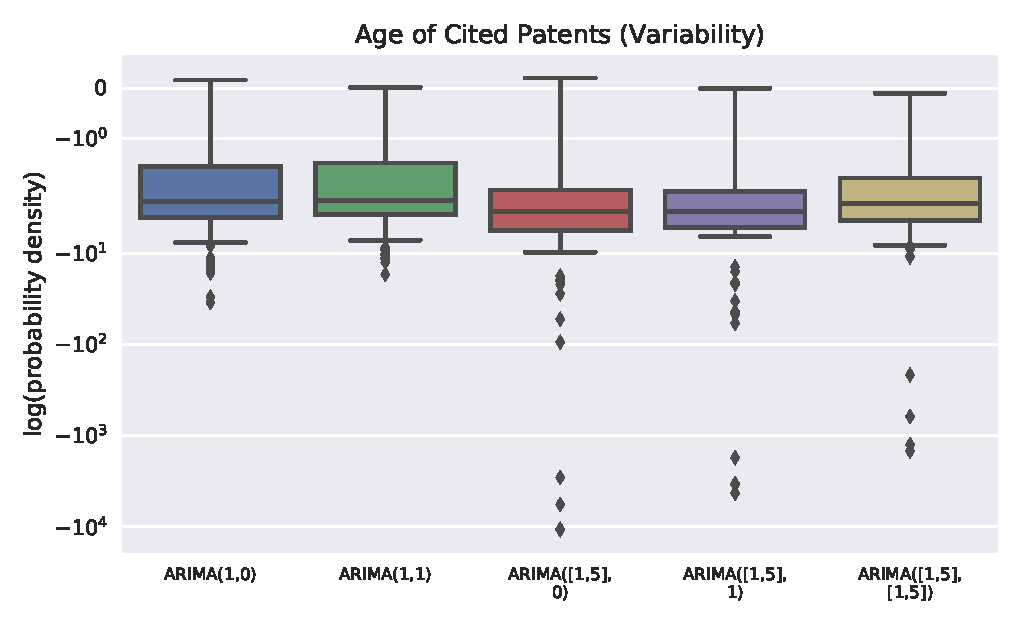
\includegraphics[width=.75\textwidth]{figs/VAR_Model_Prediction_Citations_Backward_Age_STD_Performance.pdf}
    \caption{\textbf{Distribution of forecasts' accuracies for different models of technology performance, using associated patents' variability of age of cited patents.}}
    \label{VAR_Model_Prediction_Citations_Backward_Age_STD_Performance}
\end{figure}

\begin{figure}
    \centering
    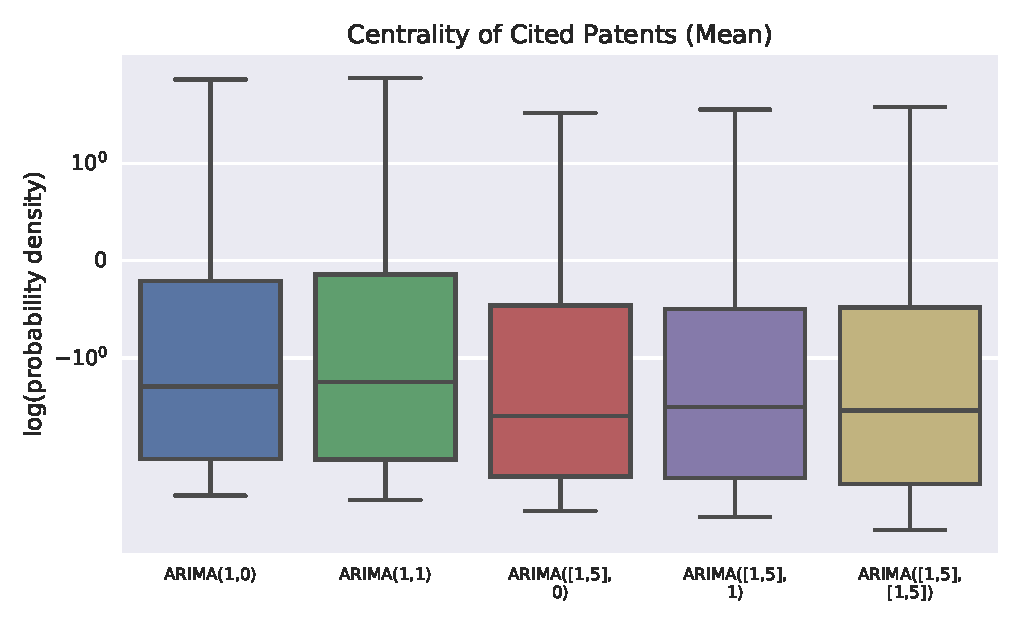
\includegraphics[width=.75\textwidth]{figs/VAR_Model_Prediction_meanSPNPcited_1year_before_Price.pdf}
    \caption{\textbf{Distribution of forecasts' accuracies for different models of technology price, using associated patents' mean centrality of cited patents.}}
    \label{VAR_Model_Prediction_meanSPNPcited_1year_before_Price}
\end{figure}

\begin{figure}
    \centering
    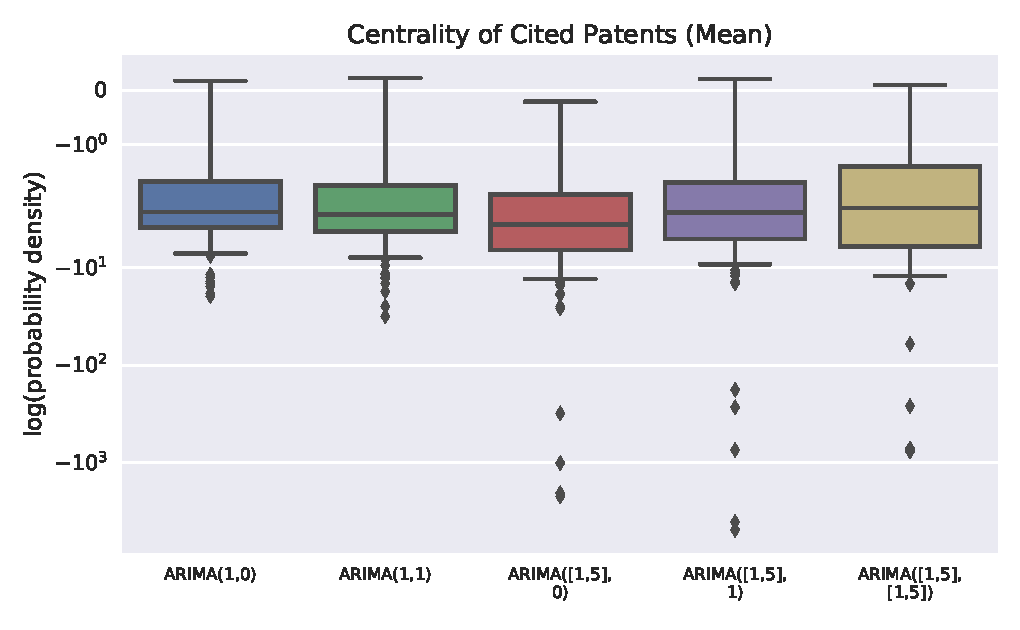
\includegraphics[width=.75\textwidth]{figs/VAR_Model_Prediction_meanSPNPcited_1year_before_Performance.pdf}
    \caption{\textbf{Distribution of forecasts' accuracies for different models of technology performance, using associated patents' mean centrality of cited patents.}}
    \label{VAR_Model_Prediction_meanSPNPcited_1year_before_Performance}
\end{figure}

\begin{figure}
    \centering
    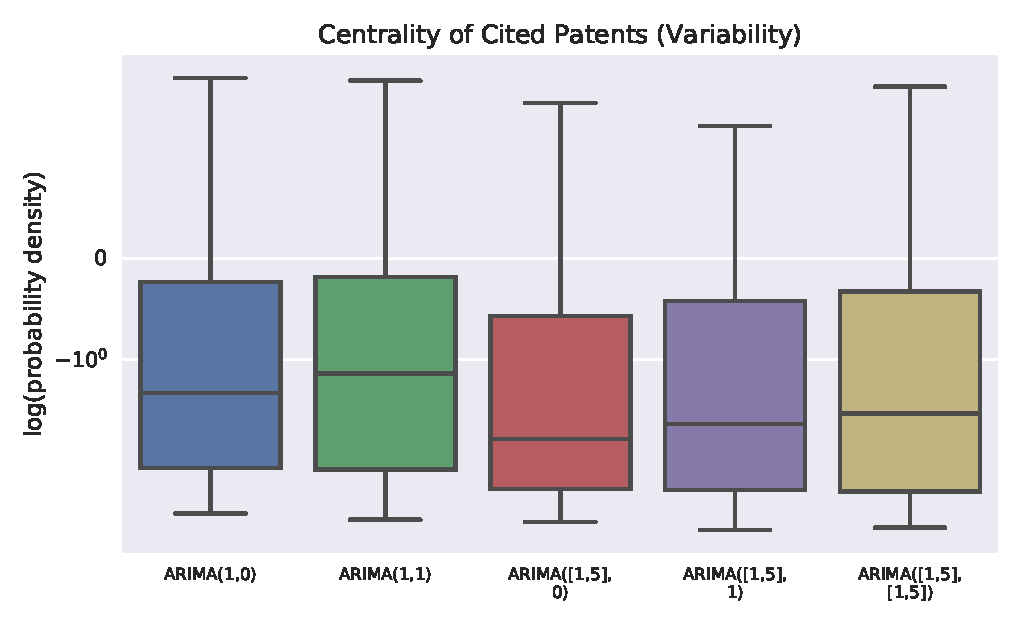
\includegraphics[width=.75\textwidth]{figs/VAR_Model_Prediction_stdSPNPcited_1year_before_Price.pdf}
    \caption{\textbf{Distribution of forecasts' accuracies for different models of technology price, using associated patents' variability of centrality of cited patents.}}
    \label{VAR_Model_Prediction_stdSPNPcited_1year_before_Price}
\end{figure}

\begin{figure}
    \centering
    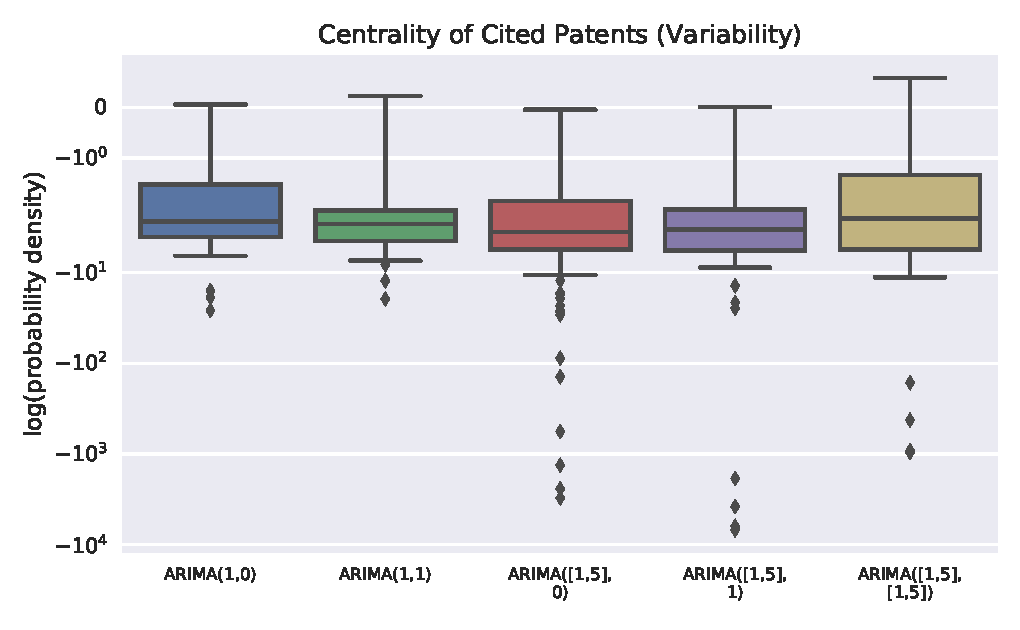
\includegraphics[width=.75\textwidth]{figs/VAR_Model_Prediction_stdSPNPcited_1year_before_Performance.pdf}
    \caption{\textbf{Distribution of forecasts' accuracies for different models of technology performance, using associated patents' variability of centrality of cited patents.}}
    \label{VAR_Model_Prediction_stdSPNPcited_1year_before_Performance}
\end{figure}

\subsection{Software}
In order to perform the analyses in this study, we wrote a statistical software package in Python named \verb$pystan_time_series$. The code for this package is freely available online at \url{https://github.com/jeffalstott/pystan_time_series}. The package uses Bayesian inference to fit time series models to data, allowing for a wide variety of options to add on to a basic ARIMA model. The package uses \verb$stan$\footnote{\url{http://mc-stan.org/}} for the inference, and uses the \verb$pystan$\footnote{\url{https://pystan.readthedocs.io/}} interface with \verb$stan$ from Python.

Additionally, all code to perform this study is available at \url{github.com/jeffalstott/technologytimeseries_forecasting}. As the patent data is too large to host on Github, that data is available upon request.

\clearpage

\section{Bonus Analysis: Forecasts of AI performance on Atari games}\label{Atari_section}
During the course of this study the Electronic Frontier Foundation began a project to compile and publish historical data on Artificial Intelligence performance on various tasks.\footnote{\url{https://www.eff.org/files/AI-progress-metrics.html}} We used the trend extrapolation process described in this study to make forecasts on a portion of this data. 

We forecasted AI performance on Atari games. Atari games have been a test bed for developing new machine learning techniques, and so there is a growing data set of AI performance over time for dozens of games. The data all came from research articles describing new AI techniques, which came with both scores on a suite of Atari games and a timestamp of when the paper was submitted. 

We used the data from 49 games (253 total data points) to do trend extrapolation of the record-breaking AI scores expected until 2020. These forecasts were made with partial pooling, which allowed for making forecasts for individual games even if there is little data available for that game. For example, the game ``Montezuma's Revenge" has data for only one top score (the first-recorded score has not been beaten), and so taken by itself this lack of trend data would prohibit making a forecast. However, because we have data from all the other games, this allowed us to infer what an average improvement rate is across all games, and then use that for making forecasting for ``Montezuma's Revenge."

Modeling this Atari data likely has similar problems to modeling the performance data earlier in this study: the model assumes the performance improves relatively smoothly, while the reality has jumps and steps. Again, the model doesn't try to capture the probability of there being no improvement on a given year. At best, it models what the record breaker's value will be, conditional on it showing up. 

But this Atari data is even more complex than the earlier performance data, in that it is clear that the AI researchers aren't even trying to set records, per se. Instead, the researchers are developing many new AI techniques and are showing off what they can do on a pre-existing suite of games. Sometimes a technique will set a new record on a game, but that wasn't the goal. The discrepancy in goals is made particularly clear by the fact that often the new AI techniques being advertised could be combined, but they are not. Instead, the articles seek to report the performance of the new technique in isolation. An ecosystem of researchers that were truly trying to push the scores on the Atari games as high as they could go would likely yield different results. Accurately forecasting record breakers does not necessarily require considering all this internal complexity, but there is ample opportunity to experiment with slightly more complex models\footcite{Berdahl2017} in the pursuit of better prediction of technology performance.


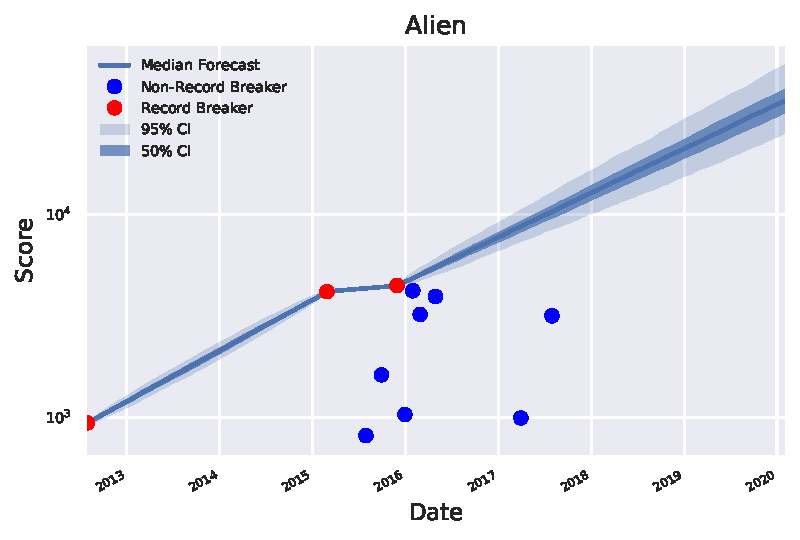
\includepdf[pages=-]{figs/Atari_Forecasts.pdf}

\end{document}